\chapter{A primer on bayesian inference}
This chapter serves as a practical introduction to bayesian data analysis using Stan, a probabilistic programming language implementing the Hamiltonian Monte Carlo (HMC) algorithm. After
introducing the core concepts of Bayesian probability, the chapter presents Markov Chain Monte Carlo algorithms,
explaining how and why they are used to define and fit statistical models. The following section describes some of the
available methods to control for the proper functioning and convergence of a Markov chain, while the next reviews how to
validate a model by testing the goodness of fit, assessing the robustness to different choices of priors, and comparing it with other models. The chapter concludes with the introduction of
multilevel models, providing two examples.

\section{Core concepts}
\subsection{Priors, likelihoods and posteriors}\label{sub:pmp}
While the mathematical concept of probability can be derived through various axiomatic formulations, it is important to recognize the distinction between its theoretical foundations and its interpretations and practical applications in statistics.
One of the primary objectives of inference is to estimate from observed data some unknown quantities, typically expressed as parameters within a statistical model.

In the frequentist interpretation, the true values of these unknown quantities are assumed to be fixed, and inference is
conducted by constructing intervals and point estimates with specific frequency properties when considering infinite
repetitions of the experiment and analysis. On the other hand, the Bayesian approach uses probability to explicitly quantify uncertainty by assigning probability distributions to these unknown parameters  \cite{d2003bayesian}.
%One of the most notable advantages of the Bayesian framework is its alignment with intuitive interpretations of statistical results. In Bayesian analysis, when estimating an unknown quantity, the outcome is presented as the actual probability distribution of the parameter.
This application of probability is not only limited to parameter estimation, and in Bayesian statistics it is possible to assign a distribution to any statement, for example allowing to determine the probability of an hypothesis.




There are several interpretations and justifications of Bayesian probability itself, with one of the most prevalent views considering it as a subjective measure of belief or knowledge in a proposition.  When inferring the value of a parameter $\theta$ based on observed data $y$, the initial knowledge about $\theta$ is quantified by its prior distribution $p(\theta)$. To carry out inference, it is also necessary to define the relationship between parameters and data, which is determined by the conditional probability $p(y|\theta)$, known as the likelihood. Once the priors and the likelihood have been established, Bayes' theorem defines the optimal way to update the knowledge about $\theta$ as follows:

\begin{equation}
p(\theta\mid y)= \frac{p(y\mid\theta)p(\theta)}{p(y)} = \frac{p(y\mid\theta)p(\theta)}{\int p(y\mid\theta)p(\theta)d\theta}
\end{equation}

The outcome of this inference step is the posterior distribution $p(\theta|y)$, while the denominator $p(y)$, referred
to as the evidence, acts as a normalization constant since it is independent of the parameters.
Central to Bayesian statistics is the concept of conditional probability, which expresses how probable an event or
statement is, given that some other event has occurred. While the likelihood represents the
probability of
obtaining some data given a specific configuration of the parameters, the posterior is the probability distribution of
the parameters once the data has been observed. Bayes' theorem defines the only way to invert the conditional relation according to the fundamental rules of
probability, allowing to obtain the posterior from the likelihood and vice-versa. Moreover, it states that doing so
requires to specify a prior distribution.


Another crucial aspect of Bayesian statistics is that the process of knowledge update can be repeated, using the
posterior as a prior for another inference step when new data is provided. If the data are independent of eachother,
progressively conditioning on partial information is equivalent to conditioning on all the
data available at the end.

The result of Bayesian inference can be identified with the posterior, which contains all of the information
resulting from the knowledge update and the priors.
Since using a full distribution to describe the results is less practical than using point estimates and intervals, the
posterior can be summarized in various ways for reporting. For instance, this can be accomplished by providing an
estimate of $\theta$ as the mean of the posterior and its standard deviation, or by computing posterior intervals
containing a certain probability, which are referred to as credible intervals.
In the Bayesian framework, credible intervals can be interpreted as containing the true value of the respective parameter with a certain
probability. This is exactly the spontaneous but erroneous interpretation commonly assigned to frequentist confidence
intervals. Given that the posterior can take on any shape and is not guaranteed to be symmetric, it is common practice
to utilize highest density credible intervals (HDI), which are defined as the smallest intervals that encompass the chosen credibility, as opposed to fixed quantiles.





\subsection{An honest discussion about priors}
While bayesian statistics have been widely adopted in the majority of social sciences, biology and medicine, until recent years
physicists have overwelminghly employed a frequentist approach in their data analysis \cite{cousins1995isn}. 
A possible partial and incomplete explanation for this difference resides in the fact that physics tend to provide very strong predictions with
specific mathematical formulas, thus very strong likelihoods, with only a handful of well specified theories being investigated most of the times.
This certainty about the underlying theory conflicts with the apparently arbitrary nature of prior distributions.
Because of this, priors can be one of the main sources of concern for a physicist approaching Bayesian statistics, as they
seem to introduce subjective elements into what should be a rigorous scientific process.

However, it should be recognized that parameter estimation and data analysis always require an additional series of assumptions on top of
those used to construct the underlying physical theory, especially when using experimental data, which is ultimately limited and
imperfect.
For example, a series of unknown quantities collectively denoted as systematics are usually introduced to
correctly account for deviations of the experimental setup from its ideal behaviour, other physical phenomenons
constituting the background, and the uncertainty on the measurements of other parameters that concurr to determine the
physical quantity that is being investigated. Moreover, the physical interpretation of many parameters requires to
impose some constraints, for example that the mass of a particle must be positive.
In most cases, complete ignorance about a parameter's possible values is rare, and experts in the field usually possess
some domain knowledge that could be useful when integrated in the analysis. It may also be of interest to start from the
results of some experiment and try to refine them with a new measurement. 

The power of priors and bayesian analysis is their ability to describe all of these assumptions in an unified
framework, by forcing to express them explicitly. Bayes' theorem
states that without priors it is impossible to conduct inference, since they are required to invert the conditional
relation between data and parameters.
Because of this central role of the priors, from now on any mention of a model will refer exclusively to the combination
of priors and likelihood. %More generally, it can be said that a model is everything that is conditioned on to compute the posterior, excluding the data.

The apparent objectivity of frequentist statistics resides in the fact that they introduce many of the underlying assumptions
implicitly
rather than explicitly. In fact, it can be shown that many common frequentist methods are particular cases of bayesian
inference with specific assumptions \cite{d2003bayesian}. Moreover, another central fact of bayesian statistics is that for well
specified models the influence of priors reduces as more data is collected, overcoming the initial subjective choices.


A useful example of how priors can be employed in physics is the treatment of systematic effects. In frequentist statistics the
analysis usually proceeds by varying the values of the systematics in a certain range and observing the consequent variation in
the results. The obtained systematic error is an additional source of uncertainty on top of the statistical error, but
there is no rigorous way to combine them. On the other hand, in a Bayesian framework a systematic is treated as any
other parameter of the model. Its expected range of variation is determined by its prior distribution, and the
additional uncertainty is automatically propagated to the posterior in the same way as the statistical uncertainty.
While it is possible to asses how much the posterior changes with the introduction of more systematics, for a given
model and data there is no way
to separate systematic from statistical error since the two are equivalent from the perspective of bayesian probability.


Priors are categorized as more or less informative based on the degree to which they restrict parameter space. 
Other than being used to model previous knowledge and systematics, they also wield significant practical influence and
can be viewed as a sophisticated regularization tool to facilitate the convergence of the algorithms employed to compute the
posterior.  Although it may be tempting to represent absolute ignorance about a parameter by assigning it a
uniform distribution over any value, this approach can lead to problematic consequences. For instance, because a flat
distribution over an infinite range cannot be normalized to 1, being denoted as improper, inference may also result in
improper posteriors, which cannot be considered probability distributions, or make their computation
unfeasible. Therefore, it is generally advisable to employ at least weakly informative but regularizing priors rather than a flat
distribution over any value. Moreover, it should be recognized that a uniform prior
is not less arbitrary than any other choice, since for a different parametrization of the model the transformed priors
do not usually remain uniform. When prior information is not available, an interesting alternative to flat distributions
is provided by the so called "objective priors", which are designed to preserve specific simmetries or useful
properties. For example, Jeffrey's priors, when combined with their corresponding likelihoods, result in posteriors
which are covariant under reparametrization \cite{objective}.
\subsection{Basic example: rate of a Poisson process}\label{sec:example}
This example will be used to show some of the previously described features of Bayesian analysis, such as how priors
can be used to constrain parameters, how the influence of priors is reduced in light of more observed data and a common
case of correspondence between bayesian and frequentist methods, at least in some asymptotic limit. Moreover, it
provides an analytical result that can be compared with those from the Monte Carlo algorithms that will be described in the next section.
\begin{figure}[t]
    \centering
    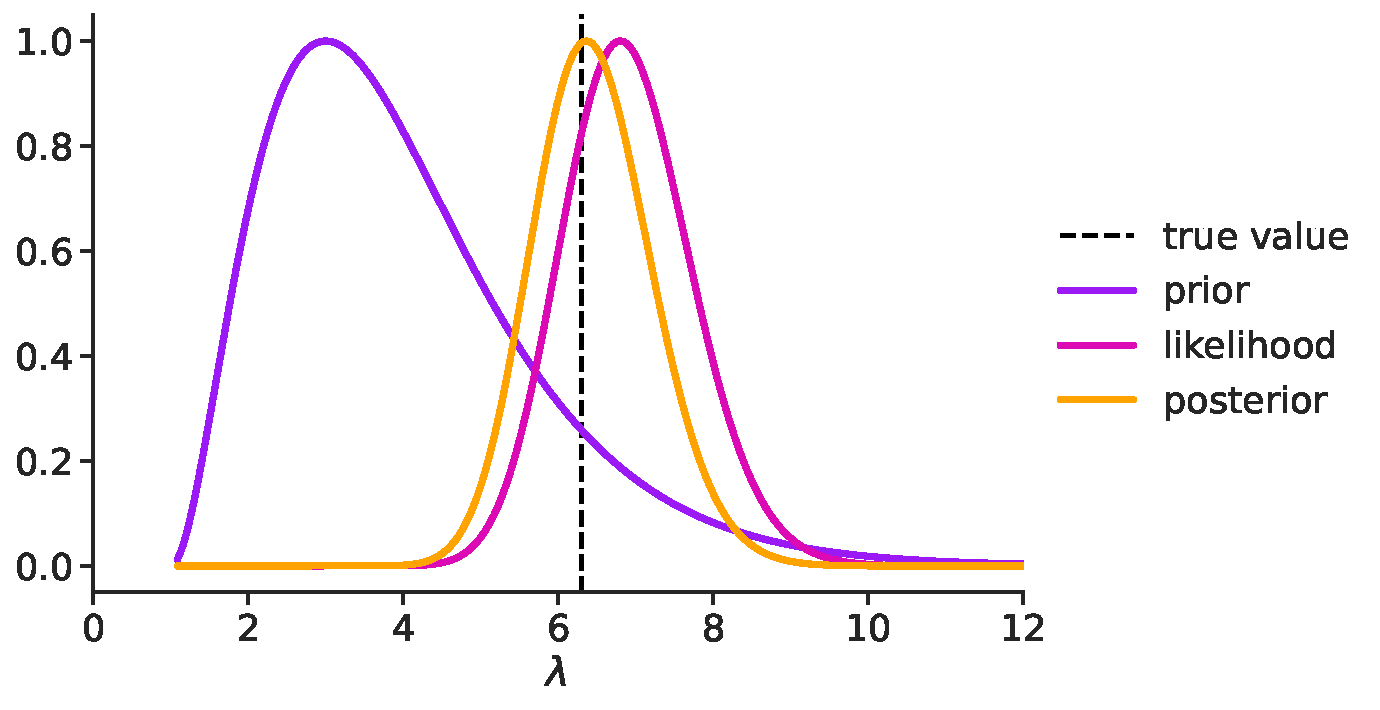
\includegraphics[width=0.9\linewidth]{figures/ch2/poisson/pdf_0.pdf}
    \caption{Analytic prior, likelihood and posterior of a Poisson rate parameter $\lambda$, obtained from $N=10$ data and a gamma prior. The distributions are not normalized.}
    \label{fig:poisexact}
\end{figure}

Consider a simple model with one parameter and a closed formula for the posterior. Given $N$ samples $y$ drawn from a
Poisson distribution, the objective is to infer its rate $\lambda$. 
Since the parameter $\lambda$ is defined as continuous and positive, this constraint can be enforced in the model by using a prior distribution that is nonzero only for positive values. A common choice for this case is the Gamma distribution, which paired with the poissonian likelihood defines the following model:
\begin{eqnarray}
    &{\mathrm{Gamma}}(\lambda|\alpha,\beta)={\frac{\beta^{\alpha}}{\Gamma(\alpha)}}\,\lambda^{\alpha-1}\,{e}^{-\beta \lambda}\\
    &\text{Poisson}(y\mid\lambda) = \prod_{i=1}^N \frac{\lambda^{y_i}}{y_i!}e^{-y_i}
\end{eqnarray}
A widespread alternative notation for statistical models, which will be used for the rest of the thesis, consists in
writing them as a series of sampling statements, denoted by $\sim$. In each sampling statement, the variable on the
left is declared as being distributed according to the function on the right-hand-side. In this case, the model can be
rewritten as:
\begin{eqnarray}
    \lambda \sim \text{Gamma}(\alpha, \beta) \\
    y \sim \text{Poisson}(\lambda)
\end{eqnarray}
It is essential to clarify that this notation only defines the functions that are used to compute the posterior. The
posterior itself will almost always be a different distribution from that used in the sampling statement of the corresponding
parameter.

While the Gamma distribution may seem as an unusual choice, in this case it allows obtaining a simple analytic expression for
the posterior. In fact, it can be shown that applying Bayes' theorem to a Gamma prior and a Poisson likelihood results
in another Gamma distribution. This property manifests for many other pairs of common distributions, known as conjugate
priors, for which the prior and the posterior belong to the same functional family \cite{diaconis1979conjugate}. For this example, the exact posterior is given by:
\begin{equation}
    p(\lambda\mid y, \alpha, \beta) = \text{Gamma}(\lambda\mid \alpha + N \overline{y},\, \beta + N)
    \label{eq:gamma_post}
\end{equation}
Where $\overline{y}$ is the mean of the data. The prior, likelihood and posterior are plotted in Fig \ref{fig:poisexact},
showing how the three components interact and provide results converging to the true rate parameter. With the analytical solution, it can be seen how the information provided by data overcomes the arbitrariness of prior choice. In fact, the mean and standard deviation of the posterior are equal to:
\begin{equation}
    \mu_{\text{post}}=\frac{\alpha + N \overline{y}}{\beta + N},\qquad     \sigma_{\text{post}}=\frac{\sqrt{\alpha + N \overline{y}}}{\beta + N},
\end{equation}
Which converge to the usual frequentist estimates $\mu=\overline{y}$ and $\sigma_\mu=\sqrt{\overline{y}/N}$ in the limit of large $N$.


\section{Markov Chain Monte Carlo}

\subsection{Integrals in high-dimensional spaces}
The current renovated interest in bayesian methods is somewhat unusual,
since bayesian statistics trace their roots in the centuries-old ideas of the founding
fathers of probability, the likes of Bernoulli, Bayes, Laplace and Gauss, while frequentists methods have become
predominant in the 20th century.
The contemporary rediscovery of Bayesian statistics is partly due to the fact that only in the last decades the necessary computational tools to tackle complex problems with a fully bayesian approach have become sufficiently powerful.
While working with a full probability density certainly is more difficult than with point estimates, the difficulty of
carrying out bayesian inference in practice may seem strange given the simple nature of Bayes' theorem, which is essentially a product of two functions.

The challenges emerge when considering models with more than one parameter. The value of the
posterior distribution can be easily computed for each point in the parameter space, but what is really needed to carry out
inference is to consider what the posterior predicts for each parameter separately. This must be done by selecting one
parameter at a time and integrating the posterior over all the others, computing what is known as the marginal
distribution of that parameter. For data $y$ and $N$ parameters $\theta_{1,\ldots N}$, the marginal posterior of the N-th parameter is given by:
\begin{equation}
    p(\theta_N \mid y)=\int d\theta_{1,\ldots N-1} p(\theta_{1,\ldots N}\mid y)
    \label{eq:marginal}
\end{equation}
For each parameter, the posterior mean, credibility intervals and all other quantities that are used for reporting and further inference must be obtained from the corresponding marginal posterior.
Since in modern applications statistical models can easily contaicolorsn thousands of parameters, it becomes essential to
address the feasibility of these integrals. 

Efficient computational methods seek to avoid unnecessary regions of parameter space which provide minimal contributions to the desired result.
An intuitive approach would be to focus on regions where the integrand is maximized, corresponding to those around the mode of
the distribution that must be marginalized. However, this overlooks a critical detail: the accumulation of integral
values requires consideration of both the probability density and the volume of parameter space.
This is due to the fact that a distribution alone only defines the density of probability for each point. The actual
probability of an event occurring in a specific range of values is given by the integral of the distribution over that range.

One of the characteristic properties of high-dimensional spaces is that there is much more volume outside any given neighborhood than inside of it.
This means that for probability distributions defined over spaces with many dimensions the region containing the mode, while still featuring the highest probability density, is contained in a very small volume.
As the number of dimensions increases, the region containing most of the probability shifts away from the mode, since the decreasing probability density is balanced with exponentially larger volume in the integration.

With an increasing dimension of parameter space, the tension between density and volume intensifies, resulting in a
narrowing of the regions where both of them are enough substantial to contribute significantly. This phenomenon, known as the concentration of measure, explains the inefficiency of brute force methods for computing integrals in many dimensions. For example, naive quadrature requires an exponentially growing number of evaluations as the dimensionality increases, yet is unlikely to intersect the narrow useful region that contributes significantly. 

%To provide an intuitive interpretation of this phenomenon, consider a multivariate standard normal with $N$ dimensions and centered on 0. In the N-dimensional space, the distance of any $N$-dimensional sample $x$ from the mode is  $\sqrt{\sum x^2}$. It becomes evident that the mean of this distance can only increase as dimensions are added because all contributions must be positive. In fact, the sum of squared standard normal variables is distributed as $\chi^2(N)$, and its square root follows a chi-distribution with N degrees of freedom. For large $N$, the mean $\mu$ of a $\chi(N)$ distribution is approximately $\sqrt{N-\frac{1}{2}} $, while its variance $N-\mu^2$ approaches $\frac{1}{2}$. This means that while the total mean distance of the samples from the mode increases indefinitely with dimensionality, their variance asymptotically reaches a fixed value. Consequently, the typical set becomes singular relative to the rest of the parameter space, as shown in figmiaoo.




\subsection{The algorithm}
Markov Chain Monte Carlo (MCMC) methods are a class of algorithms designed to probabilistically approximate integrals
and expectations by generating samples from the distribution that must be integrated \cite{geyer2011introduction}. A Markov chain is a sequence of
random variables $\{x_i\}$, where the probability of obtaining the next value is explicitly dependent only on the
current one. This conditional probability density is referred to as a Markov transition, denoted as $\mathbb{T}(x_{i+1} \mid x_{i})$. Starting from an initial point $x_1$, the sequence is constructed by iteratively applying this transition, each time sampling a new value that updates the position of the chain. The probability of reaching the N-th point in the sequence is given by:

\begin{equation}
    p(x_N) = p(x_1) \prod_{i=1}^{N-1} \mathbb{T}(x_{i+1} \mid x_{i})
\end{equation}
It is important to clarify that each $x_i$ is not an additional dimension or parameter, but that it is simply a point
in a possibly multi-dimensional space.

In a general Markov chain, the sequence simply explores parameter space without any particular utility for computing expectations. However, something remarkable occurs when the Markov transition preserves a certain target distribution $p(x)$, as expressed by the equation:

\begin{equation}
    p(x_{i+1}) = \int dx_{i} \mathbb{T}(x_{i+1} \mid x_{i})p(x_{i}) 
\end{equation}

This preservation property states that new samples generated by applying $\mathbb{T}$ to a series of samples from $p$
are still distributed according to $p$. Conversely, this means that the points in a Markov chain generated by this
transition will eventually be approximately distributed as $p$, regardless of the initial value. Given sufficient time,
the samples produced by the Markov chain enable to compute unbiased estimates for the expectation value of any function
$f$ over $p$. This is done by averaging $f$ over the Monte Carlo samples:

\begin{equation}
    \hat{f}_N = \frac{1}{N} \sum_{i=1}^N f(x_i)
\end{equation}

As the number of samples $N$ approaches infinity, these estimates converge to the true expectation $\mathbb{E}_p[f]$. 
A central aspect of this approach is the fact that expectations over the marginal distribution of a parameter are obtained simply by considering all the samples according to that parameter and discarding the dependence from the others, allowing to approximate the problematic integrals of Eq \ref{eq:marginal} in an efficient way.

In practice, achieving this asymptotic behavior is often infeasible due to limited computational resources. Thus, it is more pragmatic to consider the behavior of a Markov chain for a finite number of samples, which can be divided into three distinct phases when exploring the target distribution.
First, the chain converges from its starting position towards the region containing most of the probability defined by
the distribution $p$, leading to highly biased estimators. Second, immediately after entering that region, the exploration becomes much more efficient, rapidly reducing bias. Finally, the chain continues to refine its exploration of the distribution, resulting in slower but ongoing improvements in estimator precision. During this third phase, the estimators follow a central limit theorem:

\begin{eqnarray}
  \hat{f}^{\text{MCMC}}_N &\sim& \text{Normal} (\mathbb{E}_p[f], \sigma_{\text{MCMC}})\\
  \sigma_{\text{MCMC}} &=& \sqrt{\frac{\text{Var}_p[f]}{\text{ESS(N)}}}
\end{eqnarray}

Here, ESS (Effective Sample Size) quantifies the number of independent samples from $p$ needed to produce an equivalent
estimate. Considering that perfectly random samples must be uncorrelated, the ESS is given by the number of MCMC samples adjusted for their autocorrelation.

\subsection{Metropolis-Hastings MCMC}

The various implementations of MCMC differ in their ways to construct a transition $\mathbb T$ that ensures the
preservation property for any distribution. One commonly used method is the Metropolis-Hastings algorithm \cite{chib1995understanding}, which generates transitions through a two-step process involving proposal and acceptance. The proposal can be any stochastic perturbation of the initial state $q(x_{i+1}\mid x_{i})$. The most common choice is a gaussian distribution
\begin{equation}
  q(x_{i+1}\mid x_{i})=\text{Normal} (x_{i+1}\mid x_{i}, \sigma)
\end{equation}
On the other hand, the acceptance step is used to correct any proposals that stray too far away from the target distribution by rejecting them. The probability of accepting any proposal is given by
\begin{equation}
    a(x_{i+1}\mid x_i)=\operatorname*{min}\biggl(1,{\frac{p(x_{i+1})\,q(x_{i+1}\mid x_i)}{p(x_i)\,q(x_i\mid x_{i+1})}}\biggr)\,
\end{equation}
If the proposal is simmetric, such as in the case of the normal distribution, the acceptance probability reduces to:
\begin{equation}
    a(x_{i+1}\mid x_i)=\min \left( 1, \frac{p(x_{i+1})}{p(x_i)} \right)
\end{equation}
In contrast, asymmetric proposals find application in variants of the Metropolis-Hastings algorithm, such as Gibbs
sampling, which is widely used in statistical practice and implemented in software like JAGS \cite{plummer2003jags} and BUGS \cite{lunn2000winbugs}.

It can be shown that the Markov transitions generated by the Metropolis-Hastings algorithm preserve the target
distribution because the overall probability of the resulting Markov chain being in any $x_i$ and jumping to $x_{i+1}$ is the same as that
of it being in $x_{i+1}$
and jumping to $x_i$. This property, known as reversibility, is sufficient but not necessary to ensure the
preservation of the distribution. 

While Metropolis MCMC remains popular in many applications, its performance tends to degrade as the dimensionality of
the target distribution increases. The primary reason for this is again the concentration of measure. As the dimensionality grows,
the volume outside of the region useful for integrating the target distribution expands exponentially. Consequently, a
significant portion of proposals consists of points with extreme values in at least one dimension, leading to high rejection rates. Because of this, the Markov chain explores the distribution at an exceedingly slow pace.

In a broader context, challenges arise in all MCMC techniques when dealing with complex distributions, since the
effectiveness of a Markov transition heavily depends on their geometry. For example, in scenarios where the geometry
features narrow corners and high-curvature regions, standard Markov transitions may struggle to explore effectively,
resulting in biased estimations due to incomplete exploration. Markov chains can become trapped near the boundaries of
problematic regions, causing oscillations in the estimates that may disrupt the convergence process if the chain is
terminated prematurely. The concept of geometric ergodicity offers a formal guarantee of ideal behavior, including the
Central Limit Theorem for MCMC estimators \cite{jarner2000geometric}. However, verifying this property theoretically is challenging for all but the simplest cases, and in practice a set of empirical diagnostics is usually employed to assess the robustness of MCMC results.

\subsection{Hamiltonian Monte Carlo}
The Hamiltonian Monte Carlo (HMC) algorithm overcomes the limits of Metropolis-Hastings MCMC by generating efficient
proposals that consider the geometry of the target distribution \cite{betancourt2017conceptual}. To do so, it simulates a physical system akin to a frictionless particle subject to a potential given by the target log-likelihood function, denoted as $p(\theta)$.

In the HMC framework, each parameter of interest $\theta$ is paired with its canonical conjugate variable, denoted as $\rho$. These pairs define a joint canonical distribution $p(\theta,\rho) = p(\rho|\theta) \cdot p(\theta)$. The log-likelihood of this joint density is introduced as an artificial Hamiltonian:

\begin{align}
H(\theta,\rho) &= -\log p(\rho|\theta) - \log p(\theta) \\
&\equiv K(\rho,\theta) + V(\theta)
\end{align}

In each HMC transition, an initial momentum value is randomly drawn, initiating a trajectory which is computed through the integration of Hamilton's equations:

\begin{eqnarray}
  \frac{d\theta}{dt}& =& +\frac{\partial H}{\partial \rho} = \frac{\partial K}{\partial \rho} \\
  \frac{d\rho}{dt}& = &-\frac{\partial H}{\partial \theta} = -\frac{\partial K}{\partial \theta} - \frac{\partial V}{\partial \theta}
\end{eqnarray}

This trajectory is calculated for a fixed time, and a new point in parameter space is sampled at its endpoint, which
then serves as the starting position for the next trajectory. In this way, while the computational cost of
producing each HMC sample is quite high, the samples are guaranteed to preserve the geometry of the target distribution and feature low autocorrelation, due to the potential for the initial and final points of the trajectories to be widely separated.  The numerical integration of the trajectory employs the leapfrog integrator, which discretizes the simulation into $L$ small time intervals  $\epsilon$, interleaving half-step updates for momentum with full-step updates for position:

\begin{eqnarray}
\rho_{n+\frac{1}{2}} &\leftarrow &\rho_{n} - \frac{\epsilon}{2} \frac{\partial V}{\partial \theta}(\theta_{n}) \\
\theta_{n+1} &\leftarrow &\theta_n + \epsilon \rho_{n + \frac{1}{2}} \\
\rho_{n+1} &\leftarrow &\rho_{n+\frac{1}{2}} - \frac{\epsilon}{2} \frac{\partial V}{\partial \theta}(\theta_{n+1})
\end{eqnarray}

If numerical integration were perfect, every proposed transition would be accepted. However, the leapfrog integrator introduces a global error of order $\epsilon^2$. Fortunately, errors in numerical integration can be corrected by ensuring that the energy remains constant throughout the trajectory. This is accomplished through a Metropolis acceptance step with probability:

\begin{equation}
a(\theta_{L},-\rho_{L}|\theta_{0},\rho_{0}) = \min (1, \exp(H(-\rho_L,\theta_L)-H(\rho_0, \theta_0)))
\end{equation}

Where the inversion of the final momentum, denoted as $-\rho_L$, is required to maintain the reversibility of the
transition. While HMC is highly efficient, and proposals of well-conditioned Markov chains commonly reach acceptance rates higher than 90\%, if the simulation is not able to discretize the trajectories with sufficient precision the initial and final values of the Hamiltonian differ too much from each other, indicating that the algorithm is not correctly sampling from the distribution and leading to what are known as divergent transitions. 

To provide satisfying results, the basic version of HMC requires optimization in two key aspects:

\begin{description}
\item[Choice of Kinetic Energy:] In many applications, the momenta are sampled independently from the parameters using a
  multivariate normal distribution, $p(\rho|\theta) = p(\rho) = \text{Normal}(0, M)$, where $M$ is the Euclidean metric
  of the parameter space given by the correlation matrix between parameters. More sophisticated methods such as
  Riemannian HMC use a metric explicitly dependent on the position in parameter space.
\item[Leapfrog integrator's parameters:] while the step lenght $\epsilon$ defines the precision with which the
  trajectory is simulated, and thus the ability of properly describing the distribution, the combination of step lenght and number $\epsilon L$ determines the balance between producing long and very costly transitions or short trajectories that generate highly correlated samples.
\end{description}

Apart from the usual difficulties in exploring complex distributions with very high curvature regions, another limitation of HMC lies in its reliance on gradient-based methods, making it unsuitable for evaluating models with discrete parameters. Nevertheless, HMC can still be applied to many apparently discrete models by finding suitable reparametrizations and alternative formulations.

\subsection{No U-turn sampler and Stan}

The No-U-Turn Sampler (NUTS) is an extension of the Hamiltonian Monte Carlo (HMC) algorithm that enhances its
performance by automatically adjusting its parameters. In this implementation, the number of steps taken varies for each
transition. Instead of sequentially adding the steps of the leapfrog integrator, they are accumulated within a binary
tree of possible trajectories until one of them either turns back on itself (referred to as a "U-turn") or diverges,
with the maximum number of doublings in this tree structure being known as the tree depth. Intuitively, a U-turn occurs
when the momenta at the two extremes of the trajectory point towards each other. This implies that further extending the
trajectory would bring the initial and final points closer, resulting in a less efficient proposal due to the fact that
closer samples are more correlated.

NUTS uses an initial set of samples to achieve convergence and determine the optimal step size and metric. This phase is referred to as the "warm-up" phase. The tuned parameters are then employed for all subsequent sampling iterations. The adaptation process involves targeting a fixed acceptance rate, which is set by the user. Typically, this target acceptance rate falls between 0.6 and 0.9. Higher values lead to smaller steps and more precise trajectories but result in slower sampling due to the increased number of steps required.

Throughout this thesis, inference will be conducted using Stan \cite{carpenter2017stan}, a probabilistic programming language that implements the NUTS variation of HMC and other inference algorithms. Stan is primarily written in C++, and its language closely resembles C++. A Stan program is structured into a sequence of blocks, which are divided in seven different types:

\begin{description}
\item[Functions:] Contains a list of functions declarations and definitions to be used in the following code.

\item[Data:] The Data block is used to declare input variables. These data variables remain untransformed, and statements other than declarations are not allowed in this block.

\item[Transformed Data:] In this block, variables that do not need to change during program execution are declared. Unlike the Data Block, there's no reading from external sources; instead, it involves additional declarations and transformations of data variables. The statements in this block are executed once per chain after data is read.

\item[Parameters:] This block is used for declaring the parameters to be sampled by Stan’s NUTS implementation. These
  parameters cannot be directly assigned values and are updated at every leapfrog step of the sampler.

\item[Transformed Parameters:] This block contains additional declarations of parameters derived from the original ones
  or mixed with data variables. This block can be used to implement alternative and more efficient reparametrizations of the model.

\item[Model:] The Model block implements the actual probability model as a series of sampling statements targeting the
  parameters or the data, with all the statements concurring to define the target log-distribution that will be sampled. If priors are not explicitly defined for a certain parameter, a uniform  prior over its whole allowed range is automatically assigned to it.

\item[Generated Quantities:]This block is used for computations that do not affect the sampled parameters. It is executed each time after a sample has been generated and variables declared here are printed as part of the output. This block finds applications in generating predictions for new data, calculating event probabilities, saving the likelihood of each datapoint for model comparison and many other uses.

\end{description}

A Stan program is created by compiling a .stan model. The stanc compiler converts this model to C++ and then to an executable. The compiler and the execution of the HMC algorithm can be accessed through interfaces in various programming languages. While some interfaces provide access only to the compiler and the inference algorithms (e.g., CmdStan's command line interface), others offer additional functionality through languages like R, Python, or Julia. Among these, RStan is the most feature-rich library at the moment.
While libraries such as Rstanarm for R simplify the implementation of Stan models with pre-built functions, writing code directly in Stan allows for a deeper understanding of its inner workings and the ability to leverage its full potential. This is particularly valuable in physics applications, where models often require the implementation of specific functions and do not rely on standard classes such as linear regression.
In this thesis, all models are written directly in Stan and executed using CmdStanPy, a lightweight Python wrapper for the command line interface. Additional functions have been implemented in a Python package called "baynes", which utilizes data analysis libraries such as Seaborn and ArviZ to organize the models, plot useful graphs and aid in the execution of standard analysis routines.

\subsection{Model fitting with Stan}
Let's start by fitting with HMC the simple Poisson model of Sec \ref{sec:example}.
Here is the full implementation in Stan:
\begin{lstlisting}[language=Stan]
data {
  int<lower=0> N;
  array[N] int y;
  real alpha;
  real beta;
  int<lower=0, upper=1> prior;
}

parameters {
  real<lower=0> lambda;
}

model {
  lambda ~ gamma(alpha, beta);
  if (prior == 0){
    y ~ poisson(lambda);
  }
}
\end{lstlisting}
As can be seen, Stan allows to add constraints to the variables declarations, including parameters, which will be automatically enforced during sampling. The additional flag variable "prior" is used to switch between sampling only from the prior or from the posterior distribution when running the model without the need to recompile it.
The priors could also be checked using one of the many methods of numpy.random, scipy.stats or one of the rng functions of Stan, which would provide perfectly uncorrelated samples in less time.
Using either method is strictly a personal choice. In the examples of this thesis it has been preferred the ease of not
needing to rewrite part of the model in another language or recompile a nearly identical Stan program. Moreover,
checking if HMC struggles already when sampling from the priors allows to identify whether they are grossly
misspecified or if there are other possible problems in the implementation of the model.


\begin{figure}[t]
    \begin{subfigure}[b]{0.45\linewidth}
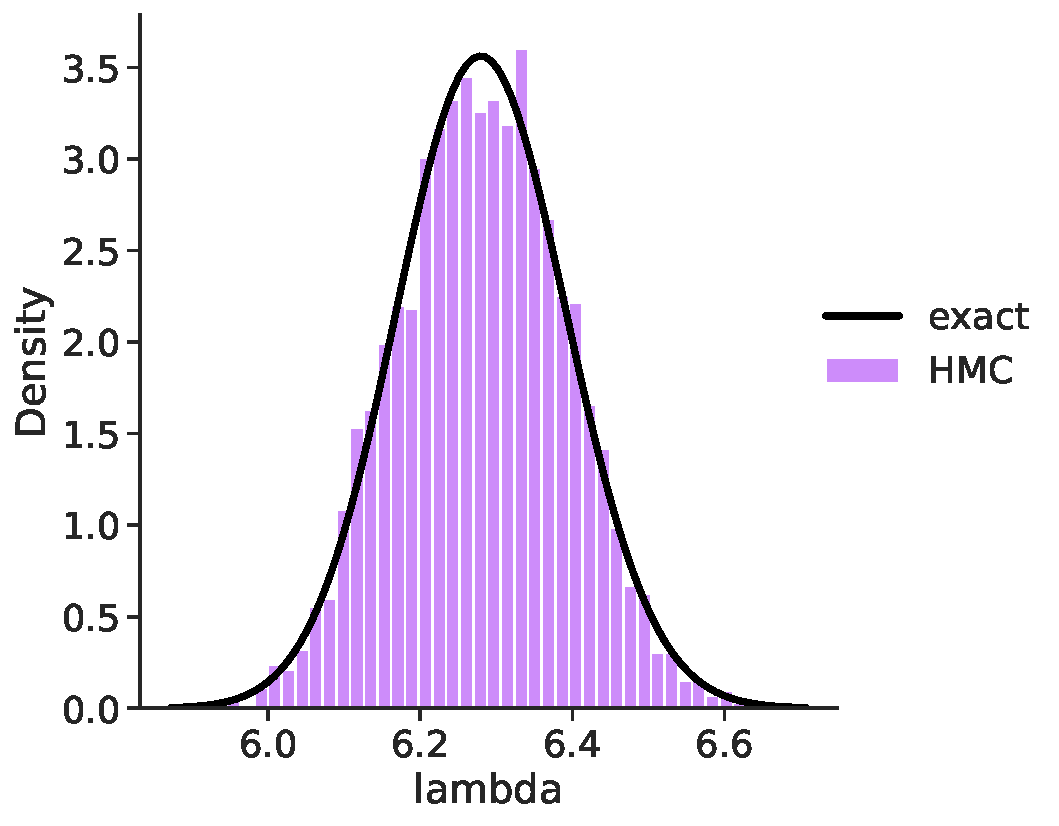
\includegraphics[width=\linewidth]{figures/ch2/poisson/plot_3.pdf}
\caption{}
\end{subfigure}
%\hfill
\begin{subfigure}[b]{0.5\linewidth}
    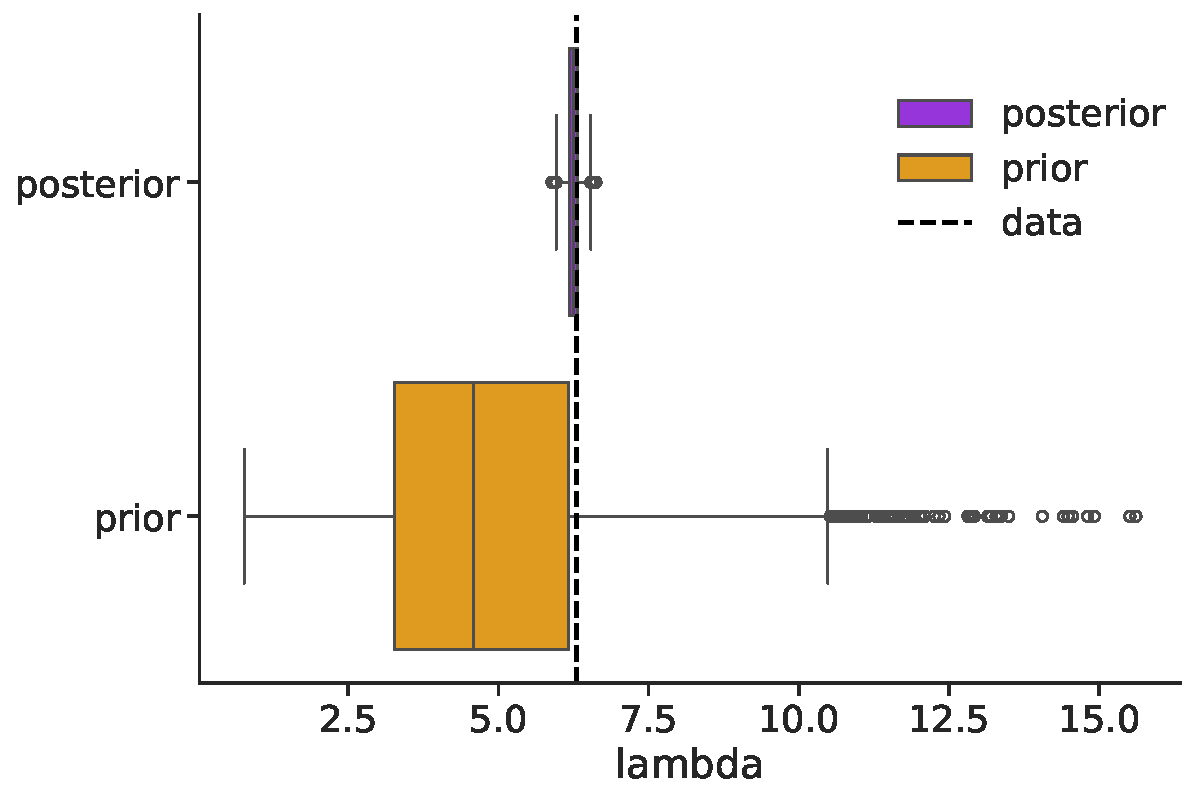
\includegraphics[width=\linewidth]{figures/ch2/poisson/cat_plot_0.pdf}
\caption{}
\end{subfigure}
\caption{Histogram of the HMC samples and analytical posterior for the rate parameter of a Poisson model (a). Boxplots of the prior and posterior HMC samples (b). } 
\label{fig:poispost}
\end{figure}

For a practical example, $N=100$ data points are generated from a Poisson with $\lambda=6.3$. Since the gamma distribution has mean $\mu=\frac{\alpha}{\beta}$ and variance $\sigma^2=\frac{\alpha}{\beta^2}$, $\alpha=5$ and $\beta=1$ are chosen to obtain a prior centered on 5 and spread between 0 and 10.
The model is compiled with CmdStanPy and fitted by running 4 chains with 500 warmup iterations and 1000 sampling
iterations each. The number of samples can be chosen depending on the precision with which the posterior estimates need
to be computed, especially for tail quantities, but this should be done considering not the raw number of iterations but the final effective sample size.

\begin{lstlisting}[language=Python]
N=100
lambda_true = 6.3
events = np.random.poisson(lambda_true, N)
data = {'N': len(events), 'y': events,
        'alpha': 5, 'beta': 1, 'prior': 0}

model = CmdStanModel(stan_file='poisson.stan')
fit = model.sample(data, chains=4,
                   iter_warmup=500,
                   iter_sampling=1000)
\end{lstlisting}



The fit results are shown in Fig \ref{fig:poispost}. The plot on the left shows an histogram of all the posterior
samples
after warmup and the exact posterior of Eq \ref{eq:gamma_post}. The two distributions provide identical estimates of mean,
standard deviation and quantiles to the third decimal place. The second plot compares the posterior and prior
distributions using boxplots, showing how much the posterior shirnks towards the true value of $\lambda$. Boxplots are a common visualization method to summarize 1-D distributions using their quartiles. The central box is given by the 25\%, median and 75\% quantiles, while the external lines extend for 1.5 quartile ranges or up to the first and last data points. Eventual outliers are plotted as single points. 

\section{Controlling the MCMC algorithm}

\subsection{HMC diagnostics}
This section will describe various diagnostics and techniques that can be applied to check for the proper working of a
Markov Chain Monte Carlo algorithm or to improve its efficiency.

While properly conditioned Markov chains are theoretically guaranteed to converge to the target distribution, this does not mean that they may do so in a reasonable time. 
The simplest way to assess potential issues with the Markov chain consists of examining the samples as a function of
each iteration, as depicted in Figure \ref{fig:pois_trace}. This graphical representation, known as a traceplot, helps
to determine whether all chains converge to the same parameter region and if they stabilize after the warm-up period.
In the case of the simple Poisson model the chains converge almost instantly, as shown in the inset which focuses on the first 50 iterations.

While traceplots are useful, they alone cannot reliably confirm the correct behavior of the Markov chains. Ensuring
their efficiency and accuracy requires various heuristics and tests since proving geometric ergodicity directly is
challenging. Fortunately, Hamiltonian Monte Carlo (HMC) offers numerous methods to assess its performance. The
"diagnose" function, accessible through every Stan interface, provides a comprehensive set of diagnostics to identify potential problems:
\vfill
\begin{figure}[t]
    \centering
    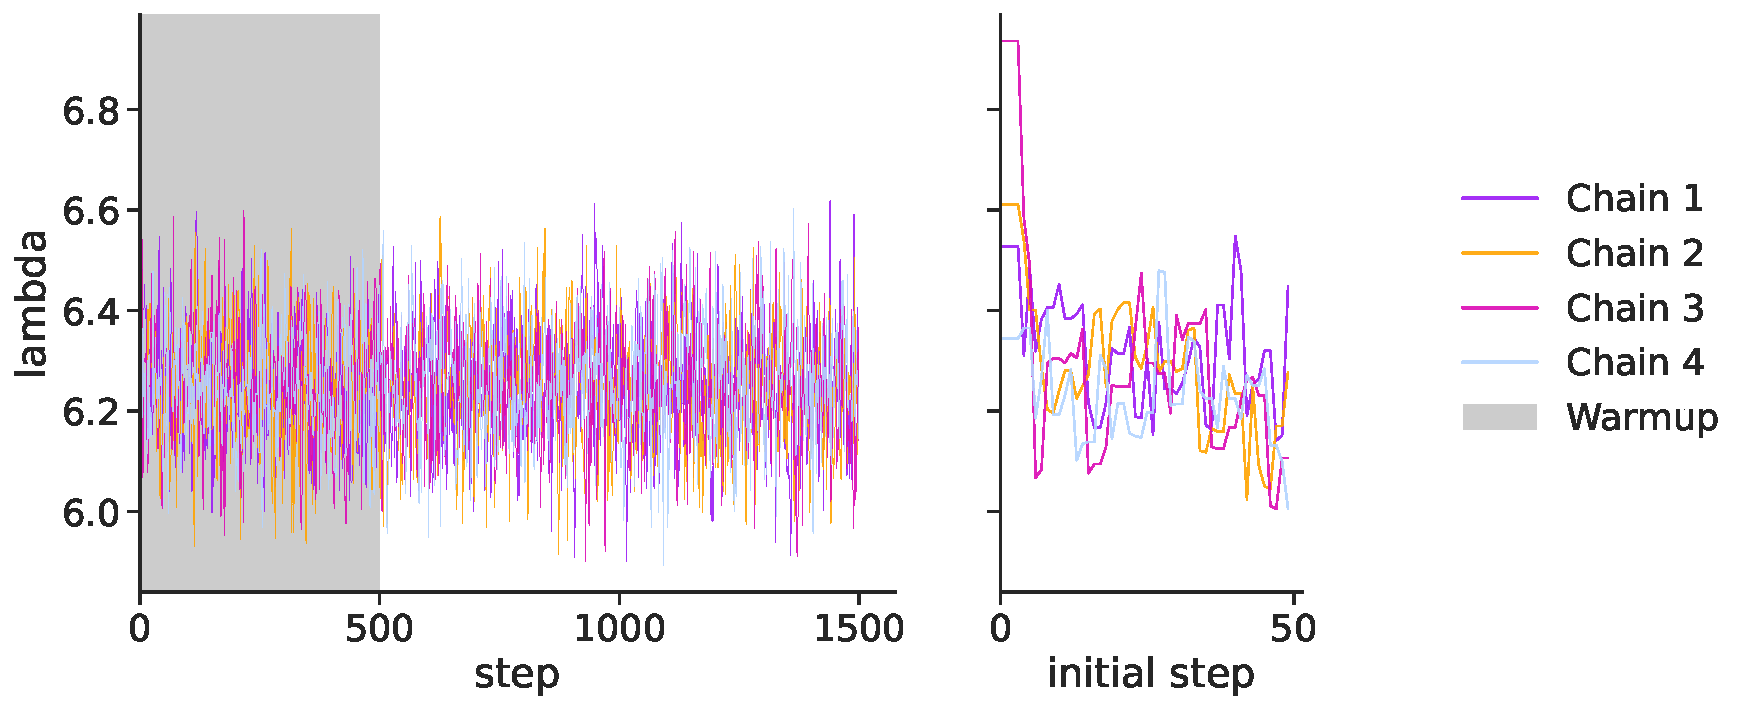
\includegraphics[width=0.9\linewidth]{figures/ch2/poisson/convergence_plot_0.pdf}
    \caption{Traceplot of the HMC chains for the rate parameter $\lambda$ of the Poisson model. The right-side plot shows how the chains rapidly converge to the posterior distributions in the first warmup iterations.}
    \label{fig:pois_trace}
\end{figure}
\vfill
\begin{description}
\item[Divergent Transitions after Warmup:] These occur when the leapfrog integrator fails to accurately approximate the
  trajectory, leading to the energy not being conserved. This issue arises when the tuned step size is inappropriate for posterior regions with complex geometry, such as narrow corners. While samples from divergent transitions are discarded and do not affect the final estimates, they indicate that the sampler struggles to explore the posterior, potentially yielding biased estimates.
\item[Maximum Treedepth Exceeded:] To prevent exceedingly long computation times, the number of branches generated by the No-U-Turn Sampler (NUTS) during each transition is capped. Hitting this limit many times typically does not introduce bias, but it signals an efficiency problem.

\item[Low E-BFMI Values:] Low values indicate inefficient exploration and high correlation among the Markov chain draws.
  This score is constructed considering that the canonical distribution $p(\rho, \theta)$ can be expressed in terms of
  energy $E$ and coordinates on an energy level $\phi$ through the microcanonical decomposition $p(E, \phi) p(E)$, with
  $p(E)$ being the marginal energy distribution \cite{betancourt2016diagnosing}. Efficient exploration requires the distribution of energies defined by momentum resampling $p(E\mid \theta)$ to closely resemble $p(E)$. The E-BFMI (Energy Bayesian Fraction of Missing Information) is the ratio of the variances of these two distributions.

\item[Low Effective Sample Size:] A low effective sample size indicates that the Markov chains are producing highly
  correlated samples, often due to very short transitions. Achieving accurate estimates, especially for extreme values,
  might require running the chain for a longer duration.

\item[High Split-$\hat{R}$:] A high Split-$\hat{R}$ score suggests that different chains have not converged by the end
  of the warm-up phase or have converged to different modes of the posterior and are not able to mix properly. The
  Split-$\hat{R}$ score is constructed by comparing the variance of all the samples together with that of each
  half-chain \cite{vehtari2021rank}.
\end{description}

To effectively diagnose sampling problems, it is highly recommended to run multiple chains from different starting
points, with a common minimum recommendation of four chains. In addition to using the $\hat{R}$ score, running multiple
chains increases the likelihood of identifying multimodality of the posterior, poor adaptation, or mixing issues.



\subsection{Reparametrization}\label{sec:repar}
As described previoulsy, Markov chain algorithms tend to perform badly when the distribution from which they extract samples has a complex shape, especially when featuring narrow corners or regions with very different scales.
Difficult geometries frustrate the HMC algorithm, leading to
slower computation times, lower effective sample size and divergent transitions. 
This problem can easily arise in models where some parameters depend explicitly from other parameters, such as those that will be described in the last section of this chapter.
A simple example is known as the
"Devil's funnel", which doesn't even require to perform inference over data but just to sample two parameters according to
the following distribution:

\begin{eqnarray}
  y&\sim&\mathrm{normal}(0,3)\\
  x &\sim&\mathrm{normal}(0,\exp(y))
\end{eqnarray}

Its fundamental characteristic is that the scale of one parameter is strongly dependent on the value of the other. Since
in HMC the optimal step size is fixed after warmup, this extreme correlation induces divergent transitions when trying to
sample in the region where the funnel becomes narrower. At the same time, selecting a very short stepsize would mean not being able to efficiently explore the broader part of the distribution.

\begin{figure}[t]
\begin{subfigure}[b]{0.31\linewidth}
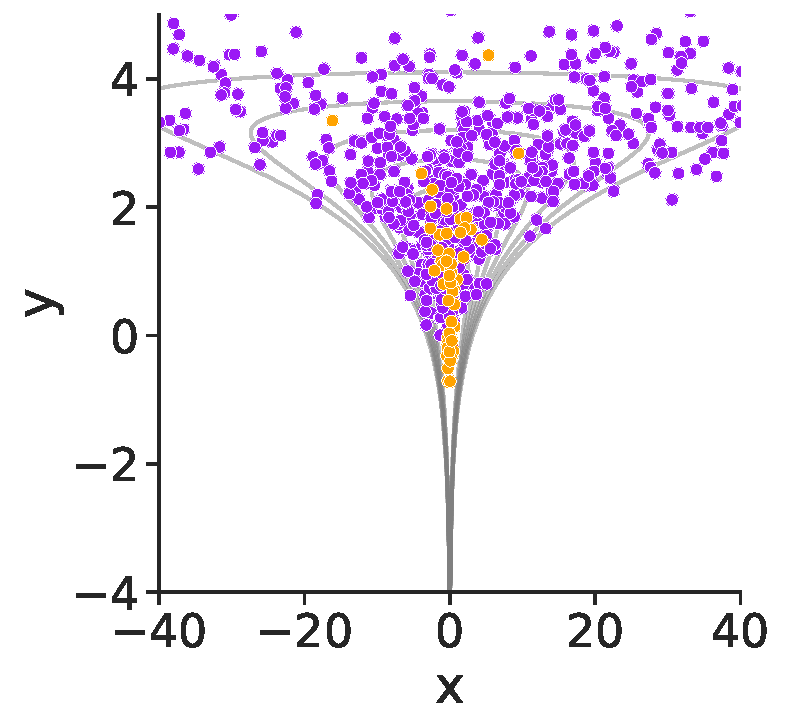
\includegraphics[width=\linewidth]{figures/ch2/poisson/funnel_0.pdf}
\caption{}
\end{subfigure}
\hfill
\begin{subfigure}[b]{0.31\linewidth}
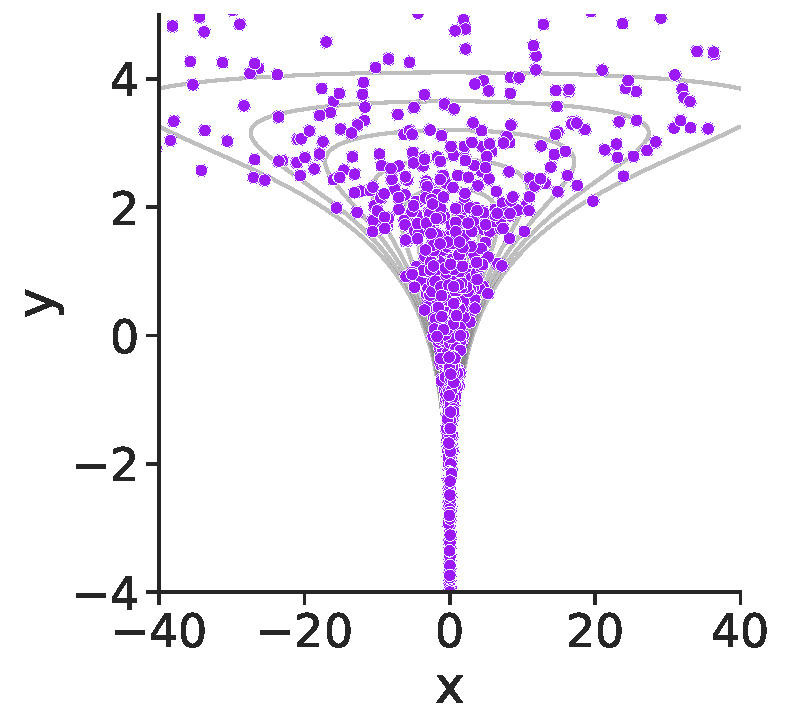
\includegraphics[width=\linewidth]{figures/ch2/poisson/funnel_1.pdf}
\caption{}
\end{subfigure}
\hfill
\begin{subfigure}[b]{0.31\linewidth}
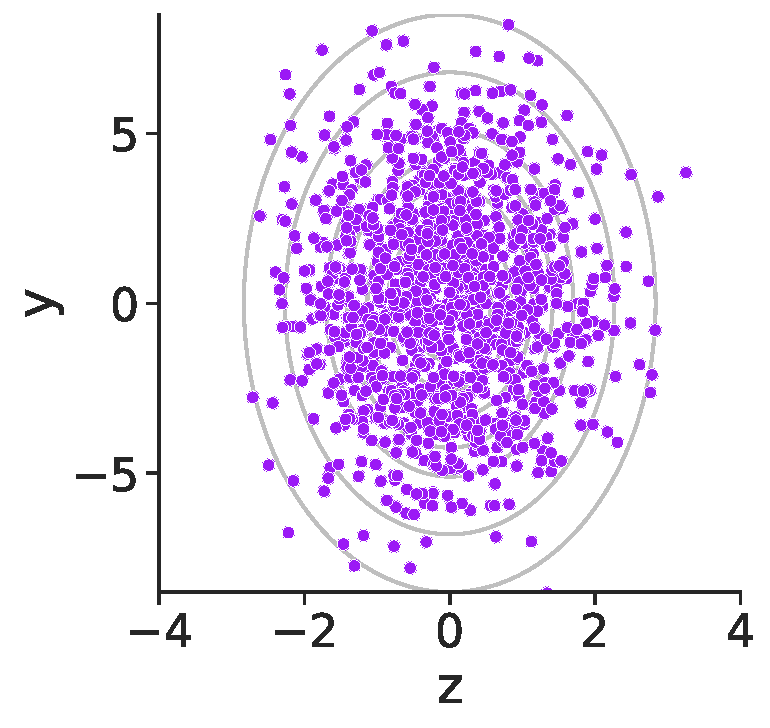
\includegraphics[width=\linewidth]{figures/ch2/poisson/funnel_2.pdf}
\caption{}
\end{subfigure}
\caption{Posterior samples for the funnel model. The centered parameterization induces divergent transitions (orange) and is
not able to explore the full distribution (a). On the other hand, the non-centered parameterization features no
divergences and is able to reach inside the funnel (b). This is because Stan is actually sampling the parameters $y$ and $z$
from normal distributions and then transforming them to $y$ and $x$ (c).}
\label{funnel}
\end{figure}
Manually adjusting the settings of the sampler will prove to be fruitless in many of these instances. In these cases, Stan's diagnostics will suggest to find an alternative parametrization.
Reparametrizing a model involves rewriting it in a different form that is mathematically equivalent but uses easier sampling statements for the algorithm. This is usually done by introducing some auxiliary parameters that are sampled according to simple distributions. These parameters can then be manipulated and combined with the others after each iteration to produce a more complex distribution without explicitly using it in a sampling statement. However, finding alternative reparametrizations is not always possible and depends upon the specific details of each model. 

The problematic implementation of the funnel where the distribution of $x$ is explicitly dependent on the other
parameter $y$ is known as a centered parametrization.
The alternative is a non-centered parameterization. Using an auxiliary parameter $z$ and leveraging the properties of the normal distribution, a non-centered
parameterization can place the embedded parameter $y$ out of the sampling statement for $x$:
\begin{eqnarray}
  y&\sim&\mathrm{Normal}(0,3)\\
  z&\sim&\mathrm{Normal}(0,1)\\
  x&=&z\exp(y)
\end{eqnarray}
Now the MCMC algorithm only needs to sample $y$ and $z$ from simple normal distributions with fixed standard deviations,
while $x$ can be computed after every iteration without needing to sample it directly.
The difference between the performance of these two parametrizations is shown in Fig \ref{funnel}.
This alternative form can be implemented in Stan using the transformed prameters block:

\begin{lstlisting}[language=Stan]
parameters {
  real y;
  vector z;
}
transformed parameters {
  vector x;
  x = z * exp(y);
}
model {
  y  ~ normal(0, 3);
  z ~ std_normal();
}
\end{lstlisting}




\subsection{Simulation-Based Calibration (SBC)}
While HMC diagnostics are a general set of tests that can be applied to all Markov chains produced by Stan and
reparametrization allows to greatly improve the sampling efficiency, these methods cannot perfectly guarantee the convergence of the algorithm. 
However, in some limited circumstances it is possible to check directly whether MCMC is sampling from the target distribution correctly.
The necessary condition for this to happen is that the data used to fit the model must be simulated from the model
itself. This is the core intuition of Simulation Based Calibration  \cite{talts2018validating}, which employs an interesting property of Bayesian models. 

Consider a process that first samples a parameter $\theta^{sim}$ from the prior distribution and then simulates data from this sample according to the likelihood of the model:

\begin{align}
\theta^{sim}&\sim p(\theta)\\
y^{sim}&\sim p(y\mid \theta^{sim})
\end{align}

Using the definition of conditional probability and Bayes' rule, it can be shown that $\theta^{sim}$ is also a sample from the posterior distribution for the simulated dataset $p(\theta\mid y^{sim})$. 
Now, consider using the same model to fit the simulated data with an algorithm such as HMC, obtaining $N$ samples of
the parameters distributed according to the posterior if the algorithm converges. Bewteen these posterior samples, count how many of them are less than $\theta^{sim}$, which is known as their rank statistic:

\begin{equation}
r(\theta^{sim}, (\theta_1\ldots\theta_N)) = \sum_{n=1}^N \mathbb I[\theta_n<\theta^{sim}],
\end{equation}

where $\mathbb I$ represents the indicator function. Since $\theta^{sim}$ and $\theta$ are obtained from the same
distribution if the algorithm is capable of correctly approximating the posterior, the ranks constructed by generating new values of $\theta^{sim}$, $y^{sim}$, and repeating the process should follow a uniform distribution from 0 to $N$. This holds true for ranks computed from any random variable over $\theta$, denoted as $f:\Theta\to \mathbb R$. 

%In this sense, Bayesian models are denoted as being inherently calibrated, providing appropriate coverage for their posterior intervals when the data is generated by the model itself with "true" parameters drawn from the priors.

It's important to highlight that this useful property is not true for any kind of data obtained from experiments, but
works only when the fit is repeated using data generated by the model itself with "true" parameters sampled from the priors.


However, this method allows isolating problems in the execution of the algorithm or validating another program used
to generate synthetic data through Monte Carlo simulation, ensuring consistency with the model. The other main
limitation of SBC is that it requires to repeat the fit multiple times, which can lead to impractical computation times
for complex models. In such cases, it may still be employed to validate the correct functioning of simpler models
before extending them with more parameters.

\begin{figure}[t]
\begin{subfigure}[b]{0.38\linewidth}
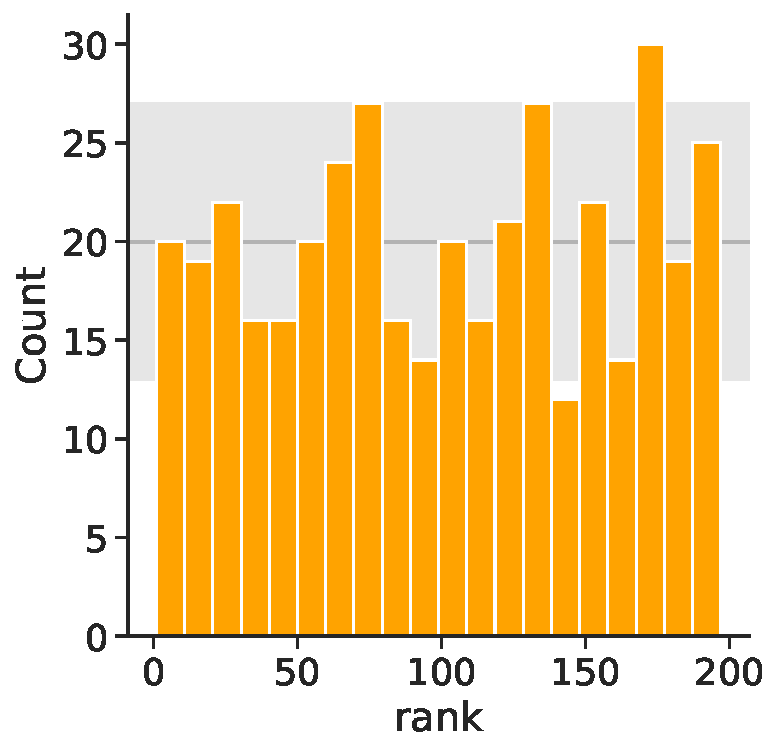
\includegraphics[width=\linewidth]{figures/ch2/poisson/SBChist_0.pdf}
\caption{}
\end{subfigure}
\hfill
\begin{subfigure}[b]{0.5\linewidth}
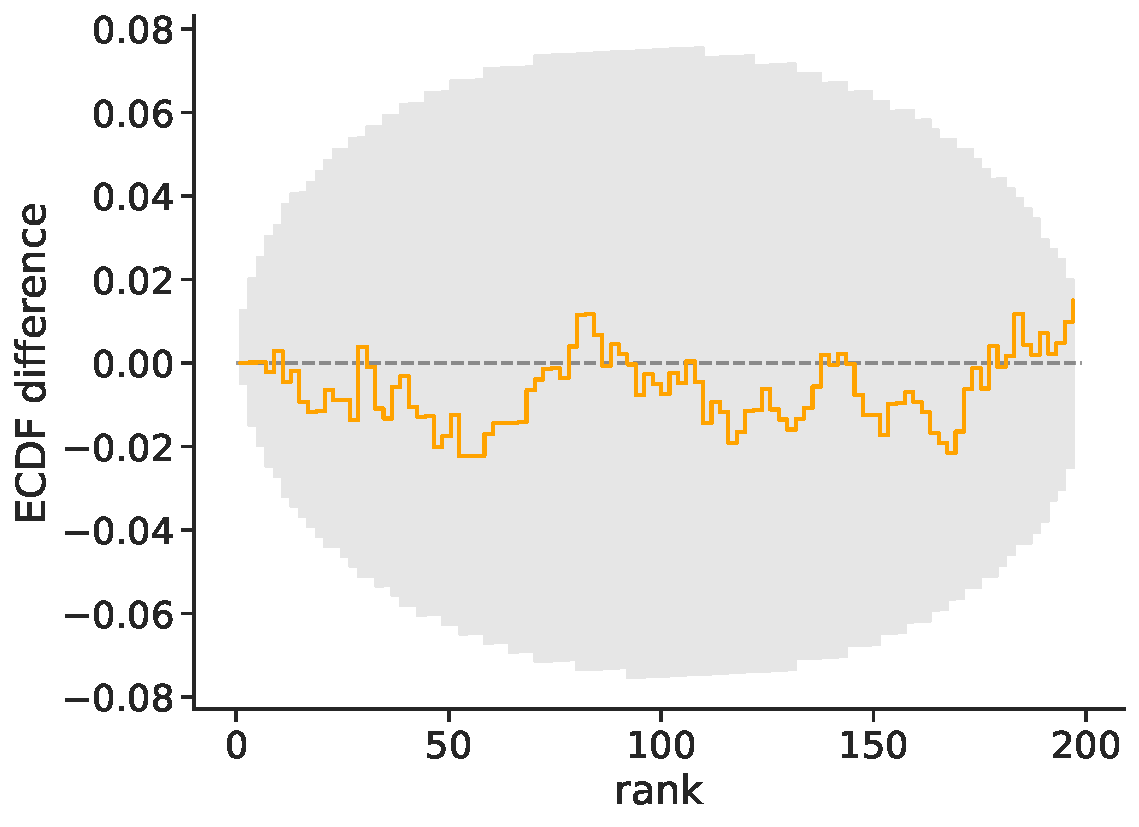
\includegraphics[width=\linewidth]{figures/ch2/poisson/SBCecdf_0.pdf}
\caption{}
\end{subfigure}
\caption{Results of SBC analysis obtained by fitting the Poisson model 1000 times, with $N=199$ samples per fit. (a) Histogram of the computed ranks for the parameter $\lambda$. (b) Difference between the ECDF of the ranks and the cumulative distribution of a uniform distribution. The grey bands represent the expected 95\% interval of possible variation assuming uniformity.}
\label{fig:poisson_SBC}
\end{figure}
SBC can be implemented within a Stan program using the transformed data block. A duplicate of the model is written in
this block, but instead of specifying a series of sampling statements, parameters and data are simulated using the
built-in RNG functions. The indicator functions, which will be accumulated into ranks, are defined within the generated
quantities block. Below is the implementation of SBC for the Poisson model, excluding the data block that is solely used
to set $\alpha$, $\beta$, and the number of data $D$:
\newpage
\begin{lstlisting}[language=Stan]
transformed data {
  real<lower = 0> lambda_sim = gamma_rng(alpha_true, beta_true);
  array[D] int<lower = 0> y = poisson_rng(rep_array(lambda_sim, D));
}
parameters {
  real<lower=0> lambda;
}
model {
  lambda ~ gamma(alpha, beta);
  y ~ poisson(lambda);
}
generated quantities {
  int<lower = 0, upper = 1> lt_lambda  = lambda < lambda_sim;
}
\end{lstlisting}
This program is executed for a total of $J$ iterations, with each iteration producing $N$ samples and a single computed
rank statistic for each parameter. %To prevent potential artifacts stemming from correlated draws, it is advisable to set $N$ close to the effective sample size ($N_{eff}$). If $N_{eff}$ is significantly lower, the chains should be sampled for a longer duration and then thinned by removing part of the samples to reduce their correlation.
The $J$ ranks can then be subjected to tests for uniformity or visually inspected using various methods. One simple
test involves accumulating the draws in a histogram with $K$ bins, where $K$ must be a divisor of $N+1$ to avoid
biases. If the expected counts per bin are sufficiently high, the distribution of counts in the histogram should follow
a chi-squared distribution with $K-1$ degrees of freedom. Alternatively, the histogram can be visualized, as shown in Figure \ref{fig:poisson_SBC} (a).

Another useful visualization method consists in plotting the difference between the empirical cumulative distribution
function (ECDF) and the expected cumulative distribution function of a uniform distribution. The ECDF at a specific
value is the proportion of samples lower than that value. The ArviZ package provides a function for plotting the
difference between the ECDF and its expected range, as demonstrated in Figure \ref{fig:poisson_SBC} (b). Visual
inspection is highly valuable, as it not only reveals whether the inference algorithm is calibrated but also how it
deviates from calibration. If the data-generating process exhibits overdispersion, underdispersion, or skewness
compared to the fitted model, these issues will be reflected in the shape of the histogram and the ECDF, which will be
significantly different from the expected range of variation.




\section{Model validation and comparison}
\subsection{Predictive checks}
The last section showed various methods for controlling the output of a MCMC algorithm and check if it has worked
properly, or to
improve its performance in order to make it correctly sample from the posterior defined by a model and the observed data.
Obtaining positive results from these procedures still does not imply anything about the ability of the model to actually describe the data, nor its usefulness. For
example, it may be extremely sensitive to priors or small variations in the underlying assumptions, or there may be
another model that generates better predictions. Different methods to address these questions will be the scope of this section.

Some of these techniques may appear unusual in the context of the standard data analysis carried out in physics, which in
many cases only requires to fit a well specified model or to
test an hypothesis. This is due to the fact that they have been developed for general applications in many other
sciences, in which it is often difficult to define a very precise theoretical model. The resulting methods are more
oriented towards model building, extending inference to a broader data analysis workflow \cite{gelman2020bayesian}. A comprehensive Bayesian workflow encompasses a sequence of interconnected
steps, from data collection and cleaning to model specification, model fitting, model expansion, and ultimately,
interpretation and decision-making. Each of these steps plays a critical role in ensuring the integrity and robustness of the analysis, aiming to capture the underlying data-generating process. 


Usually, the immediate step after controlling the convergence of a fit procedure consists in evaluating the goodness of fit.
In Bayesian data analysis, this proceeds in a way similar to Simulation Based Calibration, by simulating fake data using
the model itself \cite{gelman2013bayesian}.

When fitting a model by sampling from its posterior, the likelihood is used to compute the probability of observed data in relation to the
parameters. At the same time, in each iteration the sampled parameters define a distribution of potential new data through that same likelihood. 
Randomly sampling from the likelihood at each step of the Markov Chain generates a set of simulated data which reflects the
variability of the parameters. Notably, this simulation does not require to perform inference, but
only to sample fake data from the likelihood with an RNG function, given the parameters obtained by the Markov Chain at
that iteration.
%In this context, every Bayesian model is generative, enabling the computation of predictions by simulating data in a
%process that can be considered as "running in reverse" the likelihood.
This procedure is commonly referred to as a predictive check. Predictive checks serve as a means to evaluate whether
the model can effectively capture relevant characteristics of the data, either through visualization or by comparing
test statistics computed from the replicated datasets with those derived from the observed data. In most cases,
predictive checks are obtained from the priors or the posterior:


\begin{figure}[t]
\begin{subfigure}[b]{0.45\linewidth}
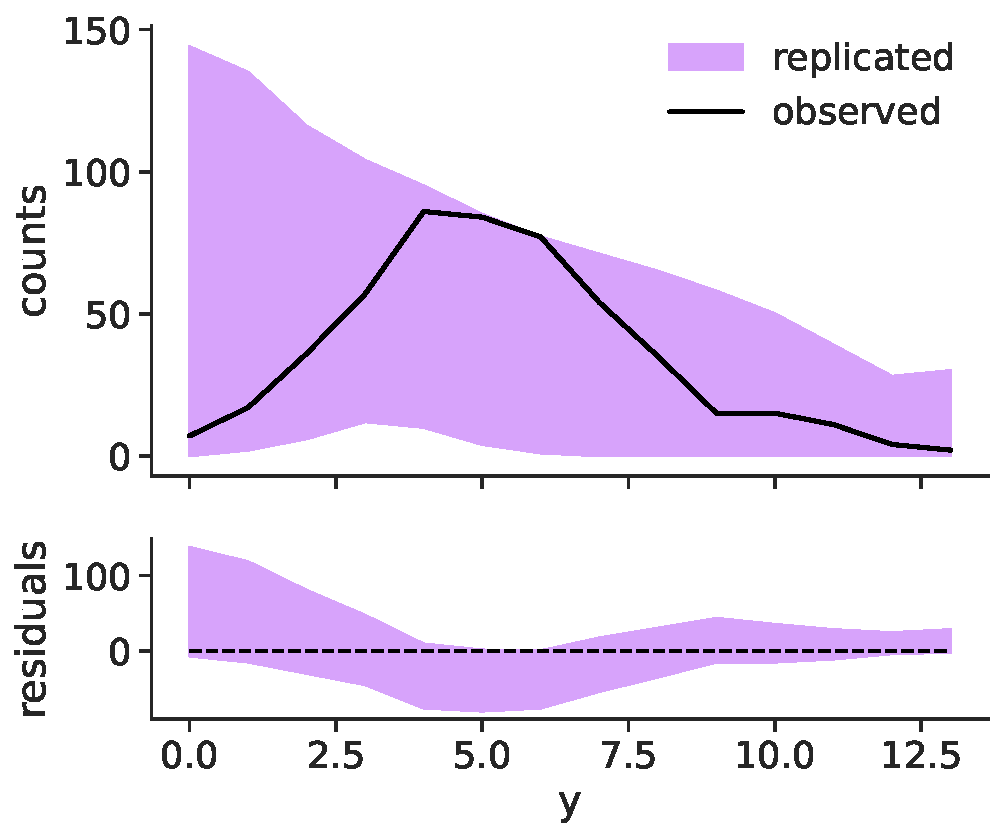
\includegraphics[width=\linewidth]{figures/ch2/poisson/predictive_check_0.pdf}
\caption{Prior Predictive Check}
\end{subfigure}
\hfill
\begin{subfigure}[b]{0.45\linewidth}
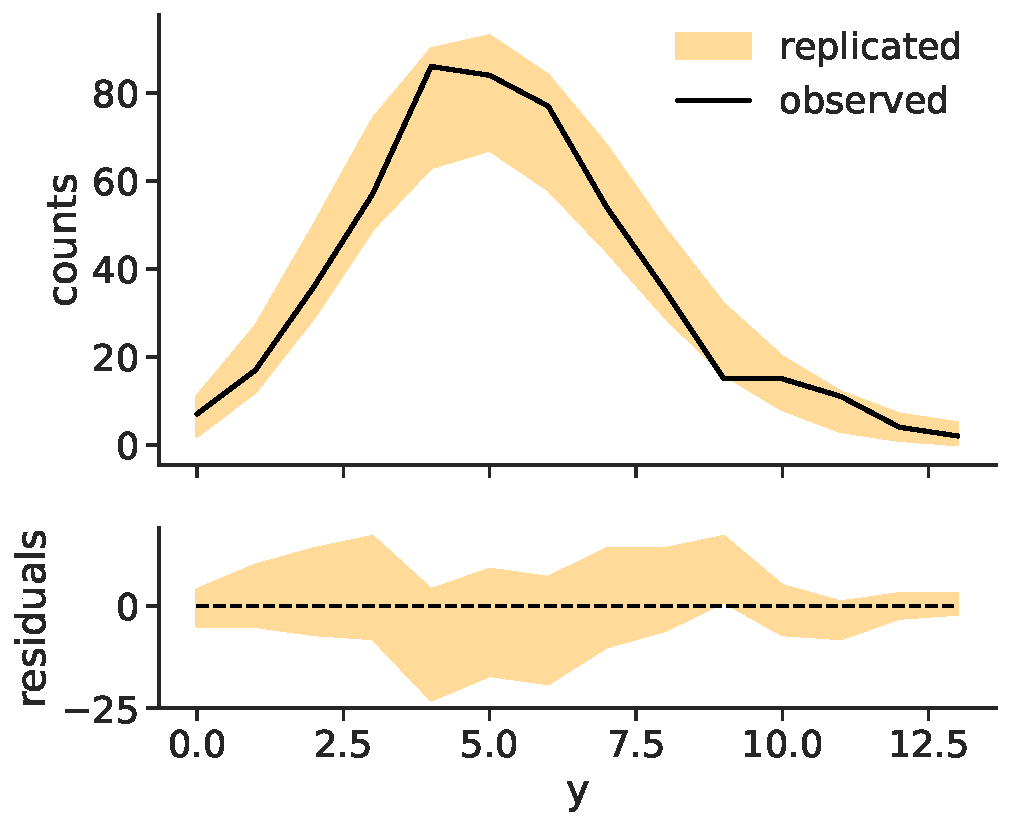
\includegraphics[width=\linewidth]{figures/ch2/poisson/predictive_check_1.pdf}
\caption{Posterior Predictive Check}
\end{subfigure}
\caption{Predictive Checks for the Poisson Model, showing the 95\% HDI of the replications of the original data $y$.
  Prior predictive check, generating sparse but reasonably distributed predictions around the data without
extreme values (a). Posterior predictive check, showing adaptation to the data (b).}
\label{fig:pois_pc}
\end{figure}
\begin{description}
\item[Posterior Predictive Checks] use samples from the posterior distribution and are employed to assess the model's
  fit to the observed data. Given an original dataset $y$ and model parameters $\theta$, sampling replicated data from the likelihood
  using parameters obtained from the posterior corresponds to sampling
  from what is known as the posterior predictive distribution:

\begin{equation}
p(y^{\text{rep}}\mid y)=\int p(y^{\text{rep}}\mid\theta)\cdot p(\theta\mid y),\mathrm{d}\theta.
\label{eq:postpred}
\end{equation}

\item[Prior Predictive Checks] generate replications from the priors, effectively sampling from the same distribution
  as posterior predictive checks in the limit of no observed data, which in this case is denoted as prior predictive
  distribution:

\begin{equation}
p(y^{\text{rep}})=\int p(y^{\text{rep}}\mid\theta)\cdot p(\theta)\mathrm{d}\theta.
\label{eq:priorpred}
\end{equation}

  They are valuable for diagnosing issues with the priors, such as whether they might be overly vague and generate
  extreme values or, conversely, be more informative but poorly positioned and shaped.
\end{description}

Figure \ref{fig:pois_pc} presents prior and posterior predictive checks for the Poisson
model, overlaying 100 replications on top of the observed data. The distribution of residuals is also plotted to facilitate visual inspection
While data visualization is a powerful tool that should be integrated into every workflow \cite{gabry2019visualization}, there is no standardized
approach for creating informative predictive check plots, especially for more complex models. Moreover, qualitative assessment
may be supplemented with quantitative scores for batch testing and automation. As previously mentioned, this can be
achieved by calculating summary statistics such as the mean, standard deviation, or quantiles for each replicated
dataset. If the model accurately replicates the data, the resulting distributions of these statistics should cover
the values derived from the observed data. Integrating the test statistics distributions from the observed value to
infinity provides a "p-value"-like score indicative of the goodness of fit, with optimal fit being represented by $p_{fit}\sim 0.5$. It is essential to note that this "p-value" score is not calibrated in the frequentist sense and does not follow a uniform distribution.

Predictive checks are implemented in Stan using the generated quantities block. Below is an example of how predictive
checks can be incorporated into the Poisson model discussed in the previous sections. The mean and standard deviation of each replicated dataset are also included in the output to be used as test statistics.

\begin{lstlisting}[language=Stan]
generated quantities {
array[N] int<lower = 0> y_rep = poisson_rng(rep_array(lambda, N));
real<lower = 0> mean_y_rep = mean(to_vector(y_rep));
real<lower = 0> sd_y_rep = sd(to_vector(y_rep));
}
\end{lstlisting}

By utilizing a flag data variable to switch between prior and posterior sampling, this same code can be employed for
both prior and posterior checks. Figure \ref{fig:pois_pc2} depicts the boxplots representing the distribution of the
means and standard deviations computed from each predicted dataset of Fig \ref{fig:pois_pc}, along with their corresponding p-values.
\begin{figure}[t]
  \begin{minipage}{0.6\linewidth}
    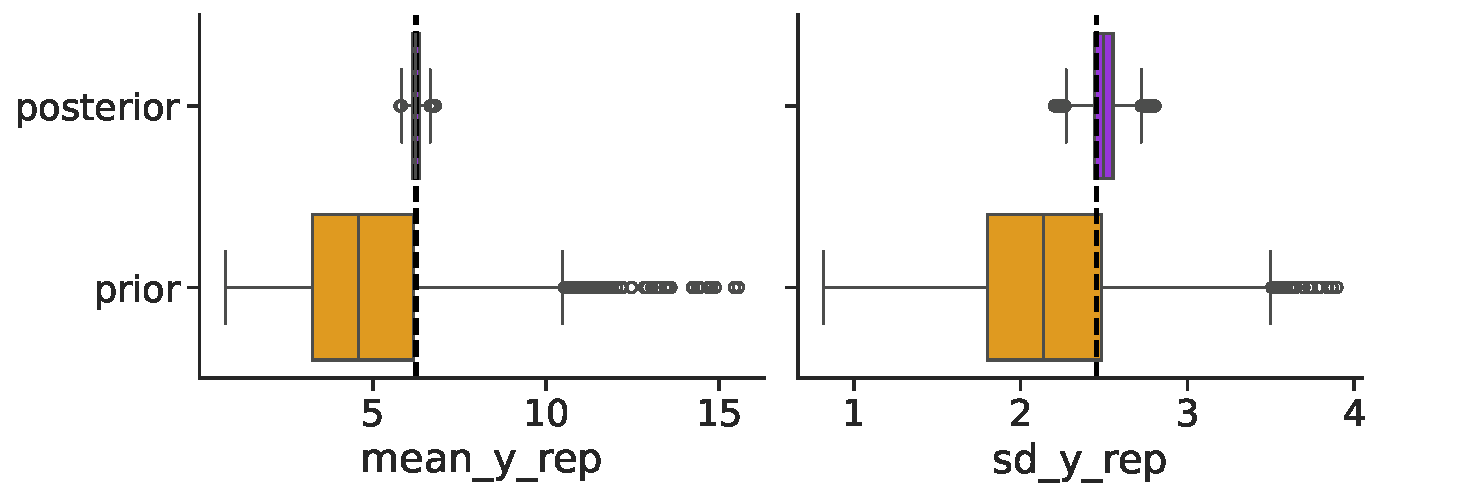
\includegraphics[width=\linewidth]{figures/ch2/poisson/cat_plot_1.pdf}
  \end{minipage}
  \hfill
  \begin{minipage}{0.4\linewidth}
    \begin{tabular}{lrr}
\toprule
 & mean\_y\_rep & sd\_y\_rep \\
\midrule
posterior & 0.50 & 0.69 \\
prior & 0.28 & 0.26 \\
\bottomrule
\end{tabular}
  \end{minipage}
    \caption{Boxplots for prior and posterior predictive checks of the Poisson model, representing the distributions for the mean and standard deviation of the replicated data, used as test statistics. The table shows their p-values.}
    \label{fig:pois_pc2}
\end{figure}

\subsection{Sensitivity analysis}
Sensitivity analysis, also referred to as robust analysis, focuses on evaluating the extent to which posterior
inferences are affected by variations in the prior, data, or model \cite{ruggeri2005robust}. 
Generally speaking, one of the most important characteristics of a model consists in the range of possible
configurations of its assumptions that determines similar results, with a more robust model producing consistent results for a wider range of variation. Due to the impossibility to choose a univocal prior distribution, prior sensititvity analysis is the major focus of these studies, which aim to determine wheter it is possible to obtain consistent results without needing incredibly specific assumptions.

The most straightforward way to gauge the influence of priors on the posterior consists in refitting the model under
different conditions and comparing the results, which is known as the informal approach. Considering the Poisson model
example, figure \ref{fig:poisson_sens} illustrates the sensitivity of the posterior distribution for the rate $\lambda$
to different choices of prior location and data count. In this case, the mean of the gamma prior $\mu=\frac{\alpha}
{\beta}$ is modified while keeping the variance fixed at $\sigma_{\text{prior}}^2=5$. The posterior medians and $95\%$ Highest Density
Interval (HDI) intervals are depicted as a function of $\mu$ and $N$. Notably, even when considering a prior centered on
$\mu=50$, which is more than 20 standard deviations away from the true value of $\lambda$, the results illustrate the
robustness of such a simple model and how the influence of priors diminishes with increasing amounts of data. These
results, obtained with Stan, are consistent from what is expected from the analytical solution of Sec \ref{sec:example}.

\begin{figure}[t]
\centering
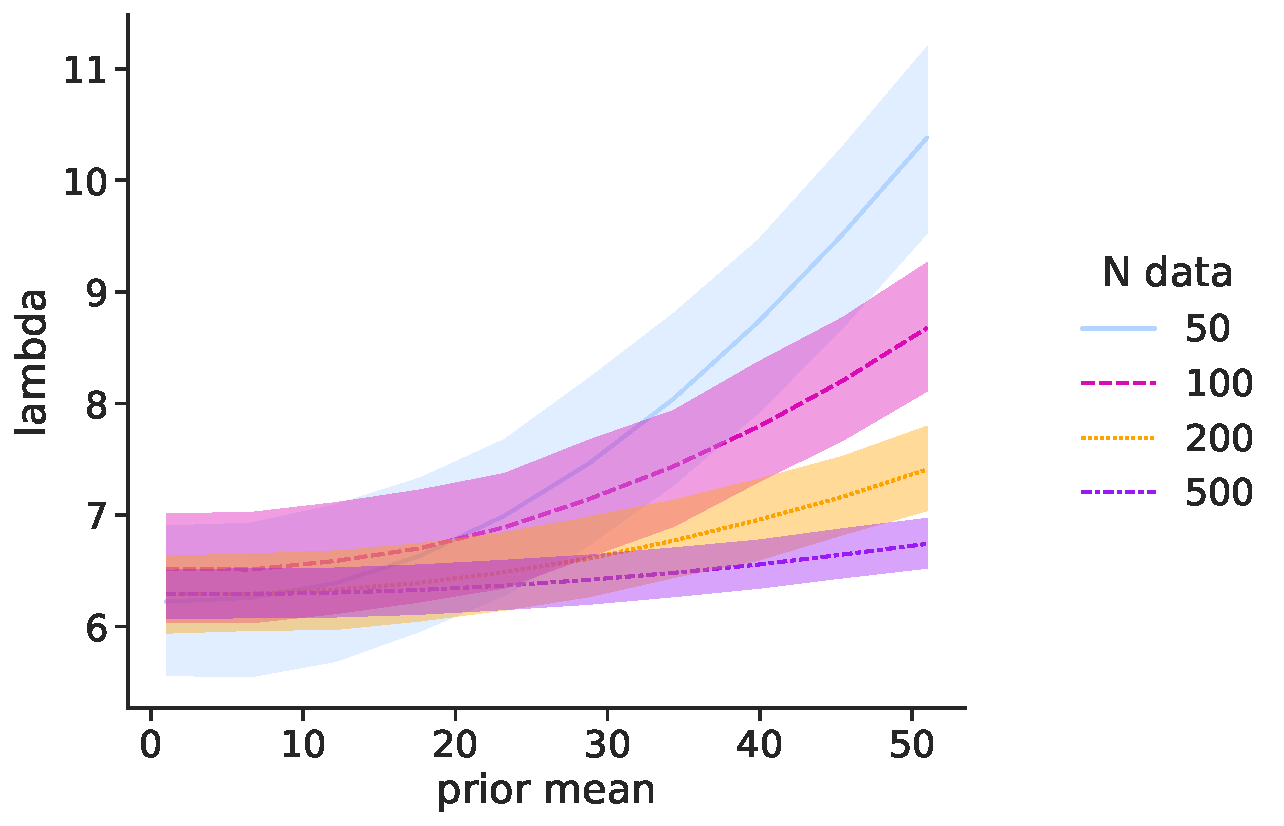
\includegraphics[width=0.85\linewidth]{figures/ch2/poisson/sens_0.pdf}
\caption{95\% HDI of posterior samples of $\lambda$ as a function of prior mean and number of data. Only the mean of
the Gamma prior is varied, while its variance is fixed to $\sigma_{\text{prior}}^2=5$. In this simple model, enough data results in stable estimates even for completely unreasonable priors.}
\label{fig:poisson_sens}
\end{figure}

Apart from the informal approach of varying the input and refitting the model, which can easily become prohibitively expensive for complex problems, there are two other main classes of prior sensitivity analysis, assessing global and local robustness respectively. 
Global robustness involves considering the entire set of priors that align with the chosen prior information using a formalized class, such as $\epsilon$-contaminated priors, where a base prior $p_0(\theta)$ is mixed with other possible choices with a probability $\epsilon$, propagating the uncertainty on priors to the posterior. The objective is to determine the range covered by the posterior mean as the prior distribution varies within this set. To achieve this, one typically identifies the extremal priors in the set, those that yield the maximum and minimum posterior means. While not requiring to fit the model for every prior in the class, this process can become intricate when dealing with multidimensional problems.

On the other hand, local robustness is interested in the rate of change in inferences, with respect to changes in the prior, and uses differential techniques to evaluate the rate. 
For example, consider a parametric class of priors $p(\theta\mid\alpha)$, which have a common functional form whose shape is determined by the quantity $\alpha$, which in this context is known as an hyperparameter. 
The local sensitivity of any expectation $f$ computed over the posterior is then given by its derivative with respect to $\alpha$ evaluated at a certain $\alpha_0$:
\begin{equation}
    \frac{\partial f(p(y\mid \theta,\alpha))}{\partial\alpha}\rvert_{\alpha=\alpha_0}
\end{equation}
Local sensitivity measures are generally more straightforward to compute in complex scenarios compared to global measures, but their interpretation and calibration may not always be as clear. 


\subsection{Hypothesis testing}
Hypothesis testing plays a central role in standard scientific practice, aiming to asses whether the observed data
provides support for a particular statement. However, it is also the subject of ongoing discussion both around its
philosophical foundations and practical implementation. While the use of p-values commonly employed in frequentist
statistics has faced significant criticism \cite{wasserstein2016asa}, at the same time Bayesian statistics offer no unified approach to hypothesis testing. 

One of the most common Bayesian hypothesis testing methods utilizes the Bayes factor (BF) \cite{kass1995bayes}. Given two competing models, denoted as $M_1$ and $M_2$, with parameters $\theta_1$ and $\theta_2$ and data $y$, the Bayes factor is defined as:

\begin{equation}
BF = \frac{p(y\mid M_2)}{p(y\mid M_1)} = \frac{\int p(y\mid \theta_1, M_1)p(\theta_1\mid M_1)d\theta_1}{\int p(y\mid \theta_2, M_2)p(\theta_2\mid M_2)d\theta_2}
\end{equation}
In this equation, the dependence on each model has been explicited in the likelihoods and priors. Each term $p(y\mid M_{i})$ in the ratio is known as the evidence, and corresponds to the normalization constant of Bayes' theorem that is usually neglected when computing the posterior with MCMC algorithms.
The Bayes factor resembles a likelihood ratio, but it averages the likelihoods over the entire parameter space rather
than using maximum values. Additionally, the BF naturally penalizes overfitting, as including more parameters expands the space over which the likelihood is averaged.

The ratio can be interpreted as providing the evidence in favor of one model over another through the probability of
observing the data, given each model. A value of $BF>1$ indicates increasing preference for $M_2$. While various scales for interpretation are cited, Bayes factors between 5 and 10 are generally considered to provide substantial evidence for $M_2$, and $BF>10$ indicates strong evidence.

However, the Bayes factor faces some critical issues. The first problem is its strong dependence on the priors of each
model $p(\theta_i\mid M_i)$. Contrary to the posterior, which usually overcomes the priors with sufficiently informative
data, the Bayes factor always remains sensitive to the details of the specified prior distributions. 
Consequently, extensive sensitivity analysis is necessary when using this method. A possible robust approach involves obtaining the lower bound of the Bayes factor for entire classes of priors instead of using a single prior distribution.

The second problem is the computational cost of integrating the likelihood over the entire parameter space to obtain the
evidence. While in some specific instances the BF can be expressed in a simpler form that allows for easier computation
\cite{heck2019caveat},
in most cases it is necessary to estimate $p(y)$ directly. Doing so accurately requires many
more ($>50\times$) MCMC samples than those used for posterior sampling, and the resulting estimates still cannot be used directly, but
must also be refined with reweighting methods like bridge sampling \cite{bridge}.

Due to these limitations, many researchers choose alternative hypothesis testing methods over the Bayes factor. One
common and simpler approach involves parameter estimation and posterior intervals. As an example, considered a specific
case of a point
null hypothesis $H_0$, corresponding to a model with one parameter fixed to certain value $\theta = 0$, while the
alternative hypothesis $H_1$ leaves $\theta$ as a free parameter. In the interval-based approach to hypotheses testing,
$H_0$ is rejected with a certain credibility $\alpha$ if the respective credible interval of the posterior distribution
for $\theta$ given $H_1$ does not contain $\theta = 0$.


The adoption of this method has sparked considerable debate, as it can yield different results than the Bayes factor for
the same data \cite{wagenmakers2020principle}. However, it can be shown that these apparent inconsistencies arise because
interval estimation implicitly assigns a prior probability of 1 to $H_1$, excluding all other hypotheses  \cite{campbell2023twofaces}. This differs from the priors used for the Bayes factor, which require both $Pr(H_1)$ and $Pr(H_0)$ to be nonzero, leading to different conclusions in many scenarios.

To reconcile these approaches, one can construct a model that encompasses both hypotheses with appropriate priors. This can be achieved using Bayesian Model Averaging, which combines samples after fitting, or by building a model with a discrete parameter that switches between the two hypotheses with a certain probability. The posterior of this discrete parameter allows to recover the Bayes factor.


\subsection{Comparing the predictive performance}
Hypotheses testing compares two models based on the evidence provided only by the observed data.
However, another possible goal of data analysis is to construct a model that is not only supported by the
available data, but also able to generate meaningful predictions. While these two approaches are closely related, the
second is especially useful in cases where specific hypotheses
cannot be established, and it is instead necessary to engage in model building and selection techniques to improve the understanding of the data generating process.
Even when all considered models exhibit mismatches with the data, it remains
valuable to evaluate their accuracy and determine potential avenues for improvement. 

The task of confronting the performance of different
models extends beyond identifying the best fit to the data, as this approach inevitably leads to overfitting. A
more robust heuristic involves assessing how a model is likely to perform on new, unobserved data, thereby automatically
penalizing overfitting. Because of this, the following comparison techniques will focus on providing a measure of the
predictive accuracy of a model.

An estimate of the disparity between models can be constructed considering the information entropy, which quantifies the
uncertainty intrinsic in a distribution \cite{mcelreath2020statistical}. For $N$ observations with respective probabilities  $p_i$, it is defined as:

\begin{equation}
    H(p)=-\sum_i^N p_i \log p_i
\end{equation}
The distance between the true data generating process defined by $p^{\text{true}}$ and the model  $p$ is then given by
the Kullback-Leibler divergence, which is closely related to the information entropy:
\begin{equation}
    D_{KL}(p^{\text{true}}, p) = \sum_i^N p_i^{\text{true}}\log p^{\text{true}}_i - p^{\text{true}}_i\log p_i
\end{equation}


This divergence can be interpreted as the additional uncertainty introduced by using $p$ to approximate
the distribution $p^{\text{true}}$. 


The central quantity involved in predictive model comparison, denoted as the "expected log pointwise predictive density" (elpd), is
constructed from the second term of the KL divergence.
The definition of the elpd considers $N$ observed data $y$ independently modeled with parameters $\theta$ and
likelihood $p(y|\theta) = \prod_{i=1}^{N} p(y_i|\theta)$, and constructs the second term of the KL divergence relative
to the distribution of unobserved data $\tilde{y}$:

\begin{equation}
\text{elpd} = \sum_{i=1}^{N}\int p^{\text{true}}(\tilde{y_i}) \log p(\tilde{y_i}|y) d\tilde{y_i}
\end{equation}
where $p(\tilde{y}|y)$ is the posterior predictive distribution of Eq \ref{eq:postpred}. Since $p^{\text{true}}$ is
usually inaccessible, it is only possible to construct a biased estimator the elpd. However, the core feature of model
comparison is that when computing the elpd for two different models the bias induced by not knowing $p^\text{true}$
is the same for both estimates, allowing for a thruthful relative comparison. 
\subsubsection*{Information criteria}
The various methods employed in model comparison mainly differ in the way the elpd estimate is constructed.
Many of the proposed approaches, historically known as information
criteria, start from the log pointwise predictive density (lpd) or a similar quantity:
\begin{equation}
\text{lpd}=\sum_{i=1}^{N} \log p(y_i|y) = \sum_{i=1}^{N} \log\int p(y_i\mid\theta) p(\theta|y) d\theta
\end{equation}
The lpd can be easily computed after obtaining $S$ draws from the posterior  $\theta_{1\ldots S}$ :
\begin{equation}
    \widehat{\text{lpd}}=\sum_{i=1}^{N}\log\left(\frac{1}{S}\sum_{s=1}^{S}p(y_{i}\mid \theta_{s})\right).
\end{equation}
However, since the lpd only considers observed data, it systematically overestimates the elpd and doesn't penalize
overfitting. To address this, a penalty term representing the effective number of parameters
$n_{eff}$ can be introduced. 
Between the many available information criteria one of the most used is the Widely Applicable Information
Criterium (WAIC) \cite{watanabe2013widely}, which is defined as:
\begin{eqnarray}
  \widehat{n}_{\mathrm{waic}} &=&\sum_{i=1}^{N}\mathrm{var_{post}}\left(\mathrm{log}\,p(y_{i}|\theta)\right),\\
   % \widehat{n}_{\mathrm{waic}} &=&\sum_{i=1}^{N}\frac{1}{S-1}\sum_{s=1}^S\left(\log p(y_i|\theta^{s})- \overline{\log p(y_i|\theta)}\right)^2\\
    \widehat{\text{elpd}}_{\mathrm{waic}} &=& \widehat{\text{lpd}}- \widehat{n}_{\mathrm{waic}}
\end{eqnarray}
As an example, consider a linear regression model with data $x$ and $y$. Vague priors are
assigned to the intercept $\alpha$, slope $\beta$ and dispersion $\sigma$: 
 \begin{eqnarray}
   \alpha &\sim&  \text{normal}(0, 10) \\
   \beta &\sim &\text{normal}(0, 10) \\
   \sigma& \sim& \text{exponential}(10)\\
   y &\sim &\text{normal}(\alpha + \beta x, \sigma)
\end{eqnarray}


Let's compare this model to a simpler version without the intercept, considering $N=20$ data simulated from
$\alpha=0.2$, $\beta=0.5$, $\sigma=0.5$. To compare Stan models using WAIC, it is necessary to add the unnormalized
likelihood for each datapoint to the output using the generated quantities block:
\begin{lstlisting}[language=Stan]
generated quantities {
  vector[N] log_lik;
  for (n in 1:N) {
    log_lik[n] = normal_lpdf(y[n] | x[n] * beta + alpha, sigma);
  }
}
\end{lstlisting}
Once the models have been fitted, the WAIC estimate of the elpd can be obtained using ArviZ, with higher elpd indicating
better predictive performance. Since an estimate can be computed for every data $y_i$, the variance between single data
estimates represents an appromixate standard error on the total computed elpd:
\begin{equation}
  \sigma_{\text{elpd}} = \sqrt{N \text{var}(\text{elpd}_i)} 
\end{equation}
When interpreting the elpd, it is then necessary not only to consider which of the models provides the highest 
value, but also if
the difference in elpd between them is significant with respect to the standard errors on the estimates. The posterior predictive checks and results for the comparison of the two linear models are shown in Fig.\ref{waic}, with WAIC favoring the inclusion of the intercept.
\begin{figure}[t]
  \begin{minipage}{0.5\linewidth}
    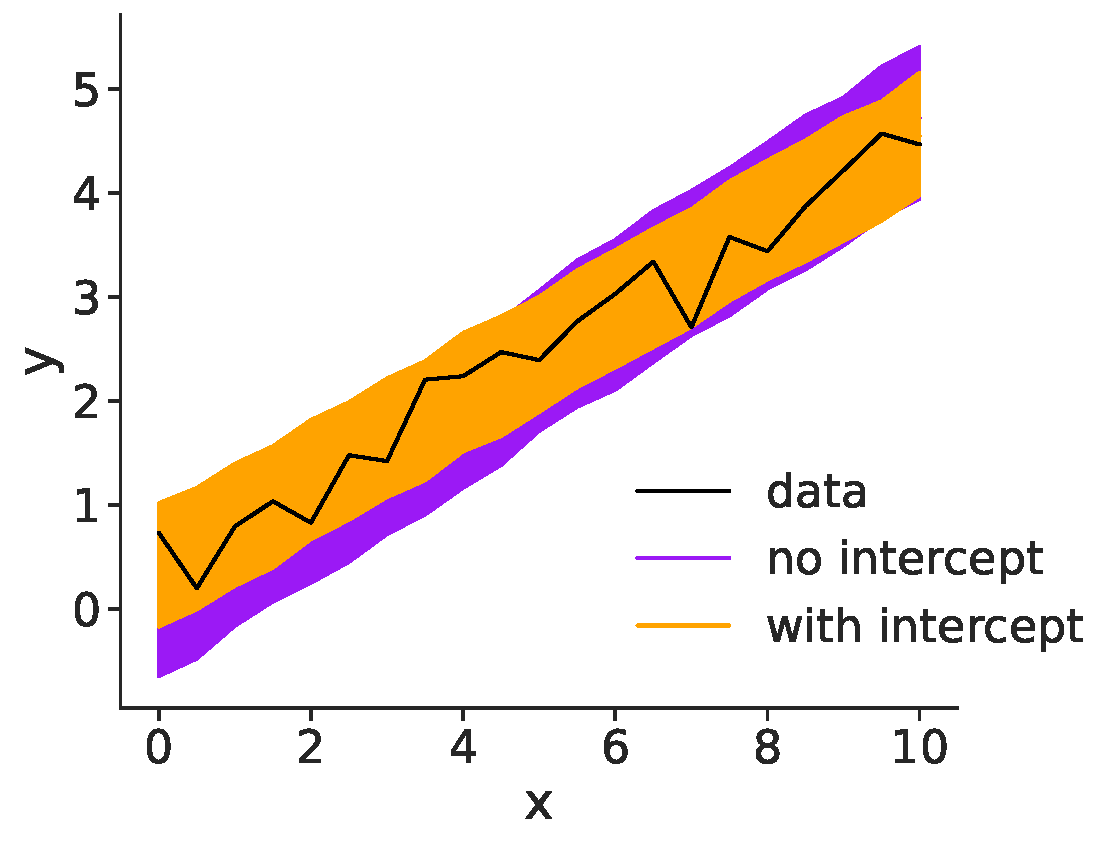
\includegraphics[width=\linewidth]{figures/ch2/linear/ppc_compare_0.pdf}
  \end{minipage} 
  \begin{minipage}{0.4\linewidth}
   \begin{tabular}{lrrr}
\toprule
 &  $elpd_{waic}$ & $\sigma_{\text{elpd}}$ & $n_{eff}$ \\
\midrule
no intercept   &      -4.6 & 2.6 &    1.4 \\
with intercept &       3.4 & 1.7 &    2.2 \\
\bottomrule
\end{tabular}
  \end{minipage}
\caption{Posterior predictive checks for linear regression models with or without intercept parameter, showing the 95\%
  highest density intervals of the replicated datasets below the observed data. The table contains the estimated elpd of each model using WAIC, its standard error and the effective number of
parameters.}
\label{waic}
\end{figure}

\subsubsection{Cross validation}
Another common strategy to asses predictive accuracy is to use only part of the data to fit the model and use the rest
to test it. To avoid discarding useful data, the sample is divided in a number of chunks, called “folds.” The
model is asked to predict each fold after training on all the others. An estimate of predictive accuracy is then
provided by averaging the scores for each fold.
Usually, only one observation at a time is excluded, implementing what is known as leave-one-out cross validation (LOOCV)
 \cite{vehtari2017practical}. With
$N$ observations and $S$ samples from the posterior, LOOCV estimates the elpd as:
\begin{equation}
    \mathrm{elpd}_{\mathrm{loo}}=\sum_{i=1}^{N}\log p(y_{i}|y_{-i})=\sum_{i=1}^N \log \frac{1}{S}\sum_{s=1}^S p(y_i\mid \theta{s,-i})
\end{equation}
Where $\theta_{s,-i}$ are samples from the posterior computed using the dataset without the i-th observation.
The key prolem with this method is that it requires to compute as many posteriors as datapoints.
Fortunately, LOOCV can be efficiently estimated using only one fit of the model over the full data. This approximation is
called Pareto smoothed importance sampling cross-validation (PSIS). Each observation $y_i$ defines a set of
weights for the full posterior samples:
\begin{equation}
  r_i(\theta_{s})={\frac{1}{P(y_{i}|\theta_{s})}}
\end{equation}
These weights are a measure of how much each observation influences the posterior. When the weights for the i-th
observation are applied to the posterior samples, the result is a set of samples resembling those from the posterior
computed without that datapoint. Reweighting the full posterior for each observation and combining the results allows
approximating the LOOCV score as:
\begin{equation}
  \mathrm{elpd}_{\mathrm{IS}}=\sum_{i=1}^{N}\mathrm{log}\,\frac{\sum_{s=1}^{S}r_i(\theta_{s})p(y_{i}|\theta_{s})}
  {\sum_{s=1}^{S}r_i(\theta_{s})}
\end{equation}

\begin{figure}[t]
  \begin{minipage}{0.4\linewidth}
   \begin{tabular}{lrrr}
\toprule
 &  $\text{elpd}_{\text{loo}}$ & $\sigma_{\text{elpd}}$ &  $n_{eff}$ \\
\midrule
no intercept   &     -4.7 & 2.6 &   1.4 \\
with intercept &      3.3 & 1.8 &   2.2 \\
\bottomrule
\end{tabular}
  \end{minipage}
  \hfill
  \begin{minipage}{0.5\linewidth}
    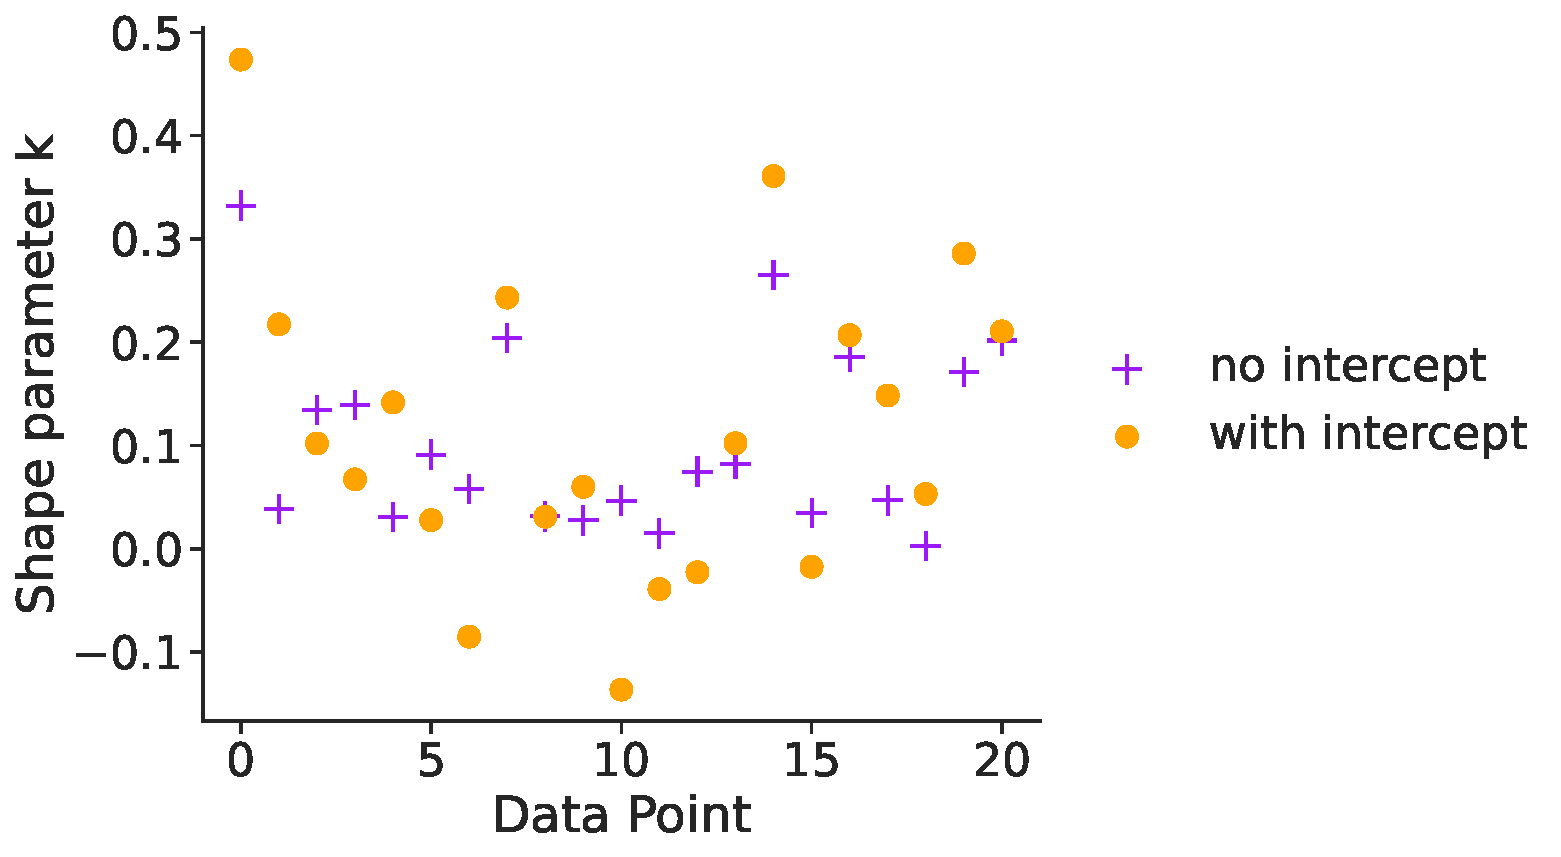
\includegraphics[width=\linewidth]{figures/ch2/linear/loo_khat_0.pdf}
  \end{minipage} 
\caption{Estimated Pareto distribution's $\hat{k}$ for each data point computed using PSIS-LOO for the linear models. All values are less than
  0.5, indicating no particularly influential data and robust approximation of the elpd. The table contains the
estimated elpd, its standard error and the effective number of parameters, with values almost equal to those obtained
with WAIC.}
\label{loo}
\end{figure}
However, this estimate is very sensitive to possible large weights due to particularly informative data, which may
introduce bias and very large fluctuations. 

The importance sampling approximation can be made more robust considering that the weights roughly follow a Pareto distribution:
\begin{equation}
  \text{Pareto}(r\mid\mu,\sigma,k)=\sigma^{-1}\left(1\ +k(r-\ \mu)\sigma^{-1}\right)^{-\frac{1}{k}-1}
\end{equation}
For each left-out observation, this distribution is fitted to the largest weights and then used to smooth extreme
values, obtaining $N$ estimates of its parameters. The shape parameter $k$ is of special interest since it provides a way to asses the reliability of the approximation. If for a certain observation $y_i$ the fit results in  $k>0.5$, the Pareto distribution has infinite variance, indicating a highly influential datapoint that may induce biased estimates.
Due to the ability of PSIS to provide feedback about its reliability and the smaller bias of LOOCV in computing the elpd with respect to WAIC,
LOOCV has become one of the primary methods for bayesian model comparison. Moreover, it can be shown that WAIC asymptotically
approaches LOO in the limit of infinite data. Beacuse of this, WAIC is still employed as a computationally easier
alternative to cross validation.

Using LOOCV with Stan also requires computing the likelihood in the generated quantities block, exactly as WAIC. The
test can also be performed using ArviZ, which provides various methods to check the approximation, for examples by
plotting the obtained shape parameters as in Fig \ref{loo}.


\section{Multilevel models}


\subsection{Measurement error}
Instead of being assigned a fixed prior, some parameters in a model can themselves be governed by a distribution dependent on other parameters. This distribution is known as a hierachical prior, and its parameters are denoted as hyperparameters. The latter also have a prior distribution, often refferred to as the hyperprior. This creates a
multilevel structure where the basic parameters can share information between each other trough the hierarchical prior,
resulting in many powerful applications that often have no frequentist counterpart, but requires some extra
considerations regarding model implementation. This final section of the chapter presents two multilevel models that could be useful
in physics applications.


The first example shows how it is possible to extend many models in order to consider data measured with a certain
error. For instance, consider $N$ data \(x_{\text{meas}}\) and $y_{meas}$, measured with known dispersions \(\sigma_x\) and
$\sigma_y$. A common task would require to fit a function $f(x)=y$ considering the error on both. In usual applications
a variant of the ordinary least squares fit is used, which however provides biased results when both the errors are significant and $f$ is nonlinear. 
Instead, the bayesian model does not approximate the relation between $x_{\text{meas}}$ and $y_{\text{meas}}$. To do so,
it introduces \(N\) parameters \(x_{\text{true}}\), representing the true values from which \(x_{\text{meas}}\) has originated. These parameters can then be given a hierarchical prior, which 
describes how the error has originated. 
The central aspect of this approach is that the hierarchical prior can describe many kinds of measurement error, not just gaussian, for example allowing to consider rounding errors or approximations in the analysis.
The true values \(x_{\text{true}}\) and eventual additional parameters in the hierarchical prior are then regularized by the respective hyperpriors. The errors on $y$ can also be modeled in different ways.

As an example, consider data measured with normal error. In this case, each \(x_{\text{meas}}[i]\) is considered to
originate from a normal distribution with mean \(x_{\text{true}}[i]\) and standard deviation $\sigma_x$. The same is
assumed for \(y_{\text{meas}}\), which will be distributed according to a normal with mean $y_{\text{true}}
=f(x_{\text{true}})$ and dispersion $\sigma_y$. In this case, the hyperprior for all \(x_{\text{true}}\) is another normal distribution used to constrain the parameters to their expected range by choosing its mean $\mu$ and deviation $\tau$. The model is specified as:
\begin{eqnarray}
x_{\text{true}} &\sim& \text{normal}(\mu, \tau)\\
x_{\text{meas}} &\sim& \text{normal}(x_{\text{true}}, \sigma_x)\\
y_{\text{meas}} &\sim &\text{normal}(f(x_{\text{true}}), \sigma_y)
\end{eqnarray}
As described in Sec \ref{sec:repar}, it is important not only to define the general form of a model, but also to
implement a specific parametrization that avoids problematic geometries in the distribution explored by the MCMC
algorithm. 
The non-centered parameterization of this measurement error model uses \(N\) standard normal parameters \(z\) instead of \(x_{\text{true}}\), improving the efficiency of the sampler:
\begin{eqnarray}
z &\sim& \text{normal}(0, 1) \\
x_{\text{true}} &= &\tau z + \mu
\end{eqnarray}

While using a new parameter for each data point may seem concerning, Stan is able to easily handle problems of this kind even with thousands of parameters. 
It is also possible to leave $\sigma_y$ as an additional parameter, however this can be done only if the error bands for \(x\) do not overlap, since this results in multiple possible valid configurations for \(x_{\text{true}}\). Finally, $\mu$ and $\tau$ can also be used as free parameters, automatically selecting the scale and position of the hyperprior.


% The second is the possibility of executing unbinned fits of convolved distributions, even when the analytic form of the convolution is not available. This may be done when \(x_{\text{meas}}\) can be sampled from a distribution that is determined by a location parameter that can be assigned to \(x_{\text{true}}\), such as the normal. In this way, \(x_{\text{meas}}\) is modeled as a sum of two random variables, with its density being the convolution between the underlying distribution of \(x_{\text{true}}\) and that of the error.


\subsection{Gaussian processes}
Gaussian processes (GP) are a bayesian machine learning technique that can be used to interpolate the available data
and generate predictions for new input values, even when no functional form is available \cite{mackay1998introduction}.
Being a bayesian method, one of their most useful properties is that they automatically quantify the uncertainty on their predictions.

The core intuition behind GPs consists in representing an arbitrary function as a series of random variables, one for
each point of the function. All of these random variables are collected in a multivariate distribution, with each variable
corresponding to an additional dimension, resulting in an infinite-dimensional distribution for continuous functions. The training data fix some points of the function, and predictions are
obtained from the correlations between these fixed points and the other variables in the many-dimensional distribution.

%This distribution can be thought of as a possibly infinite collection of random variables, each corresponding to a potential input. 

Modeling a set of output values \(f\) given their respective inputs \(x\), a Gaussian process defines this distribution as a multivariate normal with as many dimensions as there are inputs:
\[
f \sim \text{multivariate normal}(\mu(x),\Sigma(x)) \label{eq:gaussian-process} \tag{2.58}
\]
Instead of having a fixed mean and standard deviation, this multivariate normal is characterized by two fundamental components: the mean function \(\mu(x)\) and the covariance function \(\Sigma(x)\). Counterintuitively, the mean function does not significantly impact inference and can often be set to zero without loss of generality, but it will affect predictions far from any data, which will tend to be distributed around the mean. The covariance function, on the other hand, plays a crucial role, defining the distribution over functions by quantifying the correlations between different outputs as a function of the input points. It must yield a positive definite matrix for any input configuration and is often referred to as the kernel of the Gaussian process. A widely used choice is the exponentiated quadratic kernel, which produces a smooth interpolation of the data. It is given by:
\[
\Sigma(x | \alpha, \rho)_{i,j} = \alpha^2 \exp\left(-\frac{(x_i - x_j)^2}{2\rho^2}\right) \label{eq:exponential-quadratic-kernel} \tag{2.59}
\]
In this expression, \(\alpha\) and \(\rho\) represent the hyperparameters of the Gaussian process model. Intuitively,
\(\alpha\) controls the strength of the correlation between output points, resulting in smoother interpolations when
increased. On the other hand, the parameter \(\rho\) can be interpreted as the length-scale, determining the range of
the smoothing effect. Common models employing Gaussian processes combine the underlying function \(f\) with a
distribution describing how the outcomes are dispersed around \(f\). A full model specification with $N$ outcomes $y$
dispersed normally around  $f$ with standard deviation \(\sigma\), including priors for all parameters, is given by:

\begin{eqnarray} \label{eq:GP}
\rho &\sim & \text{gamma}(5,1)\\
\alpha &\sim & \text{normal}(0,1) \\
\sigma &\sim & \text{normal}(0,1) \\
f &\sim & \text{multivariate normal}(0,\Sigma(x | \alpha,\rho)) \\
y &\sim & \text{normal}(f,\sigma) \label{eq:GPfin}
\end{eqnarray}
This formulation, known as the latent variable GP, requires \(N\) parameters \(f\) to model the distribution of functions. If the outcome \(y\) is normal, as in this case, these parameters can be integrated out of the likelihood, combining the last two statements into:
\[
y \sim \text{multivariate normal}(0,\Sigma(x | \alpha,\rho) + \mathbb I_N\sigma^2) \label{eq:reduced-likelihood} \tag{2.65}
\]
This greatly reduces the computational requirements. Posterior predictive checks and the mean posterior kernel for this
model are shown in Fig \ref{fig:GP}.
\begin{figure}[t]
    \begin{subfigure}[b]{0.5\linewidth}
    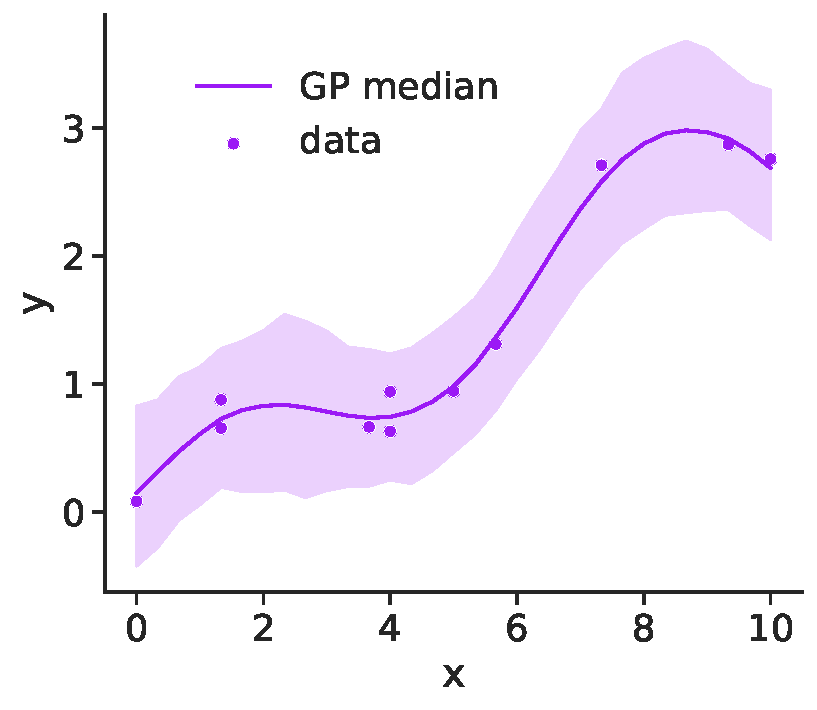
\includegraphics[width=\linewidth]{figures/ch2/GP/GP_0.pdf}
\caption{}
\end{subfigure}
\hfill
\begin{subfigure}[b]{0.5\linewidth}
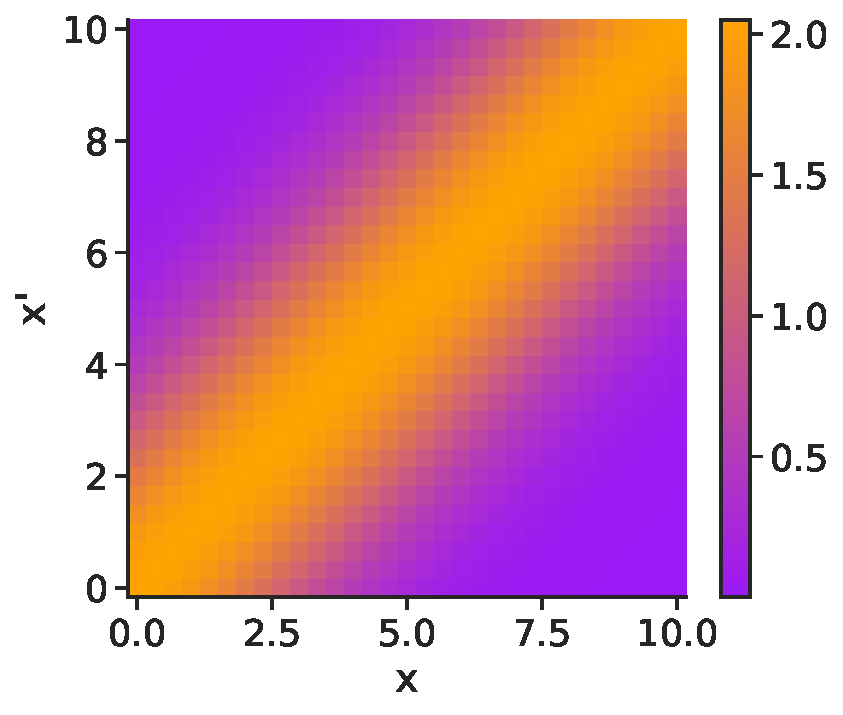
\includegraphics[width=\linewidth]{figures/ch2/GP/kernel_0.pdf}
\caption{}
\end{subfigure}
\caption{Posterior predictive check of Gaussian process regression for normal outcomes with dispersions $\sigma=0.2$, showing the median and 95\%
HDI of the predictions (a). Exponentiated quadratic kernel computed from the posterior means of the hyperparameters \(\alpha\) and \(\rho\)
(b).} 
\label{fig:GP}
\end{figure}

It is also possible to model the outcomes with another distribution dependent on the Gaussian process, for example, a
Poissonian or a Bernoulli. In this case, the latent variable formulation must be used explicitly, thus requiring a
parameter for every data point and the hierarchical structure of Eq \ref{eq:GP}-\ref{eq:GPfin}.

Implementation of Gaussian processes is commonly written in Stan using the Cholesky
factored reparameterization, which is more efficient for large datasets (\(N > 100\)). The Cholesky decomposition of
\(\Sigma(x \mid \theta)\) is the lower triangular matrix \(L\) such that \(LL^T = \Sigma\). The GP parameters \(f\)
are obtained by multiplying a vector of normally distributed parameters \(\eta\) by \(L\) and adding the mean function
$\mu$:
\begin{eqnarray}
\eta &\sim &\text{normal}(0,1)  \\
f&=&\mu + L\eta
\end{eqnarray}
Once a Gaussian process has been trained on a dataset, it becomes a powerful tool for making predictions for new input
values. The inherent uncertainty captured by the multivariate distribution provides valuable insights into the reliability of these predictions, making Gaussian processes a versatile and widely used tool both in statistics and machine learning.

